\documentclass[a4paper,12pt,twoside]{memoir}

% Castellano
\usepackage[spanish,es-tabla]{babel}
\selectlanguage{spanish}
\usepackage[utf8]{inputenc}
\usepackage[T1]{fontenc}
\usepackage{lmodern} % scalable font
\usepackage{microtype}
\usepackage{placeins}
\usepackage{eurosym}

\RequirePackage{booktabs}
\RequirePackage[table]{xcolor}
\RequirePackage{xtab}
\RequirePackage{multirow}

% Links
\usepackage[colorlinks]{hyperref}
\hypersetup{
	allcolors = {red}
}

% Ecuaciones
\usepackage{amsmath}

% Rutas de fichero / paquete
\newcommand{\ruta}[1]{{\sffamily #1}}

% Párrafos
\nonzeroparskip


% Imagenes
\usepackage{graphicx}
\newcommand{\imagen}[2]{
	\begin{figure}[!h]
		\centering
		\includegraphics[width=0.9\textwidth]{#1}
		\caption{#2}\label{fig:#1}
	\end{figure}
	\FloatBarrier
}

\newcommand{\imagenflotante}[2]{
	\begin{figure}%[!h]
		\centering
		\includegraphics[width=0.9\textwidth]{#1}
		\caption{#2}\label{fig:#1}
	\end{figure}
}



% El comando \figura nos permite insertar figuras comodamente, y utilizando
% siempre el mismo formato. Los parametros son:
% 1 -> Porcentaje del ancho de página que ocupará la figura (de 0 a 1)
% 2 --> Fichero de la imagen
% 3 --> Texto a pie de imagen
% 4 --> Etiqueta (label) para referencias
% 5 --> Opciones que queramos pasarle al \includegraphics
% 6 --> Opciones de posicionamiento a pasarle a \begin{figure}
\newcommand{\figuraConPosicion}[6]{%
  \setlength{\anchoFloat}{#1\textwidth}%
  \addtolength{\anchoFloat}{-4\fboxsep}%
  \setlength{\anchoFigura}{\anchoFloat}%
  \begin{figure}[#6]
    \begin{center}%
      \Ovalbox{%
        \begin{minipage}{\anchoFloat}%
          \begin{center}%
            \includegraphics[width=\anchoFigura,#5]{#2}%
            \caption{#3}%
            \label{#4}%
          \end{center}%
        \end{minipage}
      }%
    \end{center}%
  \end{figure}%
}

%
% Comando para incluir imágenes en formato apaisado (sin marco).
\newcommand{\figuraApaisadaSinMarco}[5]{%
  \begin{figure}%
    \begin{center}%
    \includegraphics[angle=90,height=#1\textheight,#5]{#2}%
    \caption{#3}%
    \label{#4}%
    \end{center}%
  \end{figure}%
}
% Para las tablas
\newcommand{\otoprule}{\midrule [\heavyrulewidth]}
%
% Nuevo comando para tablas pequeñas (menos de una página).
\newcommand{\tablaSmall}[5]{%
 \begin{table}
  \begin{center}
   \rowcolors {2}{gray!35}{}
   \begin{tabular}{#2}
    \toprule
    #4
    \otoprule
    #5
    \bottomrule
   \end{tabular}
   \caption{#1}
   \label{tabla:#3}
  \end{center}
 \end{table}
}

%
%Para el float H de tablaSmallSinColores
\usepackage{float}

%
% Nuevo comando para tablas pequeñas (menos de una página).
\newcommand{\tablaSmallSinColores}[5]{%
 \begin{table}[H]
  \begin{center}
   \begin{tabular}{#2}
    \toprule
    #4
    \otoprule
    #5
    \bottomrule
   \end{tabular}
   \caption{#1}
   \label{tabla:#3}
  \end{center}
 \end{table}
}

\newcommand{\tablaApaisadaSmall}[5]{%
\begin{landscape}
  \begin{table}
   \begin{center}
    \rowcolors {2}{gray!35}{}
    \begin{tabular}{#2}
     \toprule
     #4
     \otoprule
     #5
     \bottomrule
    \end{tabular}
    \caption{#1}
    \label{tabla:#3}
   \end{center}
  \end{table}
\end{landscape}
}

%
% Nuevo comando para tablas grandes con cabecera y filas alternas coloreadas en gris.
\newcommand{\tabla}[6]{%
  \begin{center}
    \tablefirsthead{
      \toprule
      #5
      \otoprule
    }
    \tablehead{
      \multicolumn{#3}{l}{\small\sl continúa desde la página anterior}\\
      \toprule
      #5
      \otoprule
    }
    \tabletail{
      \hline
      \multicolumn{#3}{r}{\small\sl continúa en la página siguiente}\\
    }
    \tablelasttail{
      \hline
    }
    \bottomcaption{#1}
    \rowcolors {2}{gray!35}{}
    \begin{xtabular}{#2}
      #6
      \bottomrule
    \end{xtabular}
    \label{tabla:#4}
  \end{center}
}

%
% Nuevo comando para tablas grandes con cabecera.
\newcommand{\tablaSinColores}[6]{%
  \begin{center}
    \tablefirsthead{
      \toprule
      #5
      \otoprule
    }
    \tablehead{
      \multicolumn{#3}{l}{\small\sl continúa desde la página anterior}\\
      \toprule
      #5
      \otoprule
    }
    \tabletail{
      \hline
      \multicolumn{#3}{r}{\small\sl continúa en la página siguiente}\\
    }
    \tablelasttail{
      \hline
    }
    \bottomcaption{#1}
    \begin{xtabular}{#2}
      #6
      \bottomrule
    \end{xtabular}
    \label{tabla:#4}
  \end{center}
}

%
% Nuevo comando para tablas grandes sin cabecera.
\newcommand{\tablaSinCabecera}[5]{%
  \begin{center}
    \tablefirsthead{
      \toprule
    }
    \tablehead{
      \multicolumn{#3}{l}{\small\sl continúa desde la página anterior}\\
      \hline
    }
    \tabletail{
      \hline
      \multicolumn{#3}{r}{\small\sl continúa en la página siguiente}\\
    }
    \tablelasttail{
      \hline
    }
    \bottomcaption{#1}
  \begin{xtabular}{#2}
    #5
   \bottomrule
  \end{xtabular}
  \label{tabla:#4}
  \end{center}
}



\definecolor{cgoLight}{HTML}{EEEEEE}
\definecolor{cgoExtralight}{HTML}{FFFFFF}

%
% Nuevo comando para tablas grandes sin cabecera.
\newcommand{\tablaSinCabeceraConBandas}[5]{%
  \begin{center}
    \tablefirsthead{
      \toprule
    }
    \tablehead{
      \multicolumn{#3}{l}{\small\sl continúa desde la página anterior}\\
      \hline
    }
    \tabletail{
      \hline
      \multicolumn{#3}{r}{\small\sl continúa en la página siguiente}\\
    }
    \tablelasttail{
      \hline
    }
    \bottomcaption{#1}
    \rowcolors[]{1}{cgoExtralight}{cgoLight}

  \begin{xtabular}{#2}
    #5
   \bottomrule
  \end{xtabular}
  \label{tabla:#4}
  \end{center}
}




\graphicspath{ {./img/} }

% Capítulos
\chapterstyle{bianchi}
\newcommand{\capitulo}[2]{
	\setcounter{chapter}{#1}
	\setcounter{section}{0}
	\chapter*{#2}
	\addcontentsline{toc}{chapter}{#2}
	\markboth{#2}{#2}
}

% Apéndices
\renewcommand{\appendixname}{Apéndice}
\renewcommand*\cftappendixname{\appendixname}

\newcommand{\apendice}[1]{
	%\renewcommand{\thechapter}{A}
	\chapter{#1}
}

\renewcommand*\cftappendixname{\appendixname\ }

% Formato de portada
\makeatletter
\usepackage{xcolor}
\newcommand{\tutor}[1]{\def\@tutor{#1}}
\newcommand{\course}[1]{\def\@course{#1}}
\definecolor{cpardoBox}{HTML}{E6E6FF}
\def\maketitle{
  \null
  \thispagestyle{empty}
  % Cabecera ----------------
\noindent
\includegraphics[width=\textwidth]{cabecera}\vspace{1cm}%
  \vfill
  % Título proyecto y escudo informática ----------------
  \colorbox{cpardoBox}{%
    \begin{minipage}{.8\textwidth}
      \vspace{.5cm}\Large
      \begin{center}
      \textbf{TFG del Grado en Ingeniería Informática}\vspace{.6cm}\\
      \textbf{\LARGE\@title{}}
      \end{center}
      \vspace{.2cm}
    \end{minipage}

  }%
  \hfill\begin{minipage}{.20\textwidth}
    
\includegraphics[width=\textwidth]{escudoInfor}
  \end{minipage}
  \vfill
  % Datos de alumno, curso y tutores ------------------
  \begin{center}%
  {%
    \noindent\LARGE
    Presentado por \@author{}\\ 
    en Universidad de Burgos --- \@date{}\\
    Tutor: \@tutor{}\\
  }%
  \end{center}%
  \null
  \cleardoublepage
  }
\makeatother


% Datos de portada
\title{Gestión desde Android de un simulador de control domótico con Raspberry Pi}
\author{Mario Juez Castrillo}
\tutor{César Represa Pérez}
\date{\today}

\begin{document}

\maketitle



\cleardoublepage



%%%%%%%%%%%%%%%%%%%%%%%%%%%%%%%%%%%%%%%%%%%%%%%%%%%%%%%%%%%%%%%%%%%%%%%%%%%%%%%%%%%%%%%%



\frontmatter


\clearpage

% Indices
\tableofcontents

\clearpage

\listoffigures

\clearpage

\listoftables

\clearpage

\mainmatter

\appendix

\apendice{Plan de Proyecto Software}

\section{Introducción}

Para llevar acabo este proyecto he seguido una metodología llamada \textit{Top-down}. 
En el modelo \textit{Top-down} se formula un resumen del sistema, sin especificar detalles. Cada parte del sistema se refina diseñando con mayor detalle. Cada parte nueva es entonces redefinida, cada vez con mayor detalle, hasta que la especificación completa es lo suficientemente detallada para validar el modelo \cite{wiki:topdown}. Teniendo como base lo anterior, la planificación que se ha seguido ha sido marcar por parte de mi tutor desde un principio los requisitos generales tanto funcionales como no funcionales que debería tener el sistema. Y a partir de esto, yo por mi parte crear requisitos a más bajo nivel según trataba de implementar sus requisitos.

\section{Planificación temporal}

En cuanto a la planificación temporal de este proyecto, no ha sido realizada por semanas, sino de la siguiente manera:

\begin{enumerate}
	\item El primer día quedé con mi tutor, y el me explicó que se esperaba del proyecto y que debería tener de cara a su exposición. De esta manera elaboramos unos requisitos generales.
	\item A partir de estos requisitos generales, siguiendo la metodología \textit{Top-down}, yo mismo cree requisitos más detallados y más pequeños que me llevarían a la implementación de los requisitos generales.
	\item Cada vez que se consiguiese un requisito general de los elaborados, se realizaría  una reunión en la que se mostraría el contenido en cuanto a código y funcionalidad de dicho requisito.
	\item En dicha reunión, se exponen mejoras estéticas o de funcionalidad para dicho requisito, ya que a primera vista son muy generales, y nos enfocamos hacia el siguiente.
\end{enumerate}

Durante la realización del proyecto se han ido siguiendo los pasos anteriores, y no se ha realizado una planificación semanal, ya que cada reunión dependía de cada requisito. Además es posible que un requisito pudiese estar resuelto en una semana, pero otro en dos, o incluso tres semanas, dependiendo de la complejidad.

A partir de los objetivos fijados, como planificación \textit{Top-down} elaboré una serie de tareas más sencillas para ir realizando y conseguir cumplir dichos objetivos. Estas son las tareas que me propuse para cumplir los objetivos y mantener cierta planificación temporal en el proyecto.

\begin{itemize}
	\item \textbf{Definir una habitación y los elementos a controlar.} 
	\begin{enumerate}
		\item Crear una \textit{Activity} o ventana principal que contendrá las estancias \footnote{estancias: posibles lugares de la casa: \textit{Habitación}, \textit{Salón}, \textit{Cocina}, \textit{Baño}}.
		\item Crear un botón para poder crear las estancias dinámicamente.
		\item Buscar una estructura para almacenar estancias en la que se permita la inserción, modificación y eliminación de ellas.
		\item Implementar la funcionalidad del botón.
		\item Crear una estructura personalizada para adaptarla a nuestras necesidades.
		\item Diferenciar a la hora de la inserción que tipo de estancia estamos insertando mediante una lista de opción única.
		\item Añadir imágenes de las diferentes estancias para que sea más visual al usuario saber que tipo de estancias ha creado.
		\item Añadir un menú contextual en la estructura que permita modificar el nombre de la estancia o su eliminación.
	\end{enumerate}
	\item \textbf{Conexión con la estación.}
	\begin{enumerate}
		\item Buscar información sobre como realizar la conexión.
		\item Implementar una conexión saliente mediante \textit{Sockets}.
		\item Implementar dicha conexión en una tarea asíncrona para mejorar su funcionalidad.
		\item Añadir dicha funcionalidad cuando se creen nuevas estancias o se modifiquen las ya existentes de alguna manera.
	\end{enumerate}
	\item \textbf{Incremento de la funcionalidad de la aplicación.}
	\begin{enumerate}
		\item Crear una \textit{Activity} o ventana secundaria donde se representará la iluminación.
		\item Crear un botón para poder crear las bombillas dinámicamente.
		\item Buscar una estructura para almacenar dichas bombillas en la que se permite la inserción, modificación y eliminación de ellas.
		\item Implementar la funcionalidad del botón.
		\item Crear una estructura personalizada para adaptarla a las necesidades de la bombilla.
		\item Implementar la funcionalidad del interruptor para cambiar el estado de la bombilla.
		\item Añadir un menú contextual en la estructura que contiene las bombillas que permite modificar el nombre de ellas y su eliminación.
		\item Permitir que se realice una conexión a la estación con la creación de nuevas bombillas o que se modifiquen las ya existentes de alguna manera.
		\item Añadir flecha de retroceso que nos devuelva a la ventana principal.
		\item Permitir que al pulsar sobre una estancia nos dirija a su ventana secundaria con su iluminación correspondiente.
	\end{enumerate}
	\item \textbf{Desarrollo de la interfaz en la Raspberry Pi.}
	\begin{enumerate}
		\item Crear una ventana básica vacía.
		\item Buscar una estructura en la que poder almacenar de forma visual las estancias y su iluminación.
		\item Crear la estructura donde se almacenarán.
		\item Añadir funcionalidad a la estructura para que permita la modificación y eliminación de las estancias y su iluminación.
		\item Crear el servidor socket para escuchar los mensajes de la aplicación.
		\item Crear un método que interprete los mensajes que llegan de la app.
		\item Separar el servidor socket en un hilo independiente.
		\item Añadir texto e imágenes en la parte de iluminación.
		\item Añadir iconos a la estancias para diferencias cada tipo.
		\item Añadir persistencia de los elementos.
		\item Añadir la introducción de la IP del servidor de forma gráfica.
		\item Modificar el servidor para que permita la conexión de más de un usuario simultáneamente.
	\end{enumerate}
	\item \textbf{Mejora de utilización de la aplicación.}
	\begin{enumerate}
		\item Crear una \textit{Activity} o ventana donde se representará la \textit{ip}, el \textit{puerto} y el \textit{estado} del servidor.
		\item Permitir la conexión y desconexión del servidor desde esta ventana mediante un botón.
		\item Mantener la persistencia de los elementos de la aplicación mediante una base de datos local.
		\item Permitir borrar la base de datos desde el menú desplegable de la ventana principal.
		\item Permitir acceder a la ventana del Servidor desde el menú desplegable de la ventana principal.
		\item No permitir realizar cambios de ningún tipo sin estar conectado al servidor.
		\item Crear un hilo independiente que escuche los cambios que nos manda el servidor.
		\item Actualizar la vista con cada cambio que nos llegue del servidor.
		\item Actualizar la base de datos local con la base de datos del servidor cada vez que nos conectemos a él.
	\end{enumerate}
	\item \textbf{Lanzamiento de la primera versión completamente funcional.}
	\begin{enumerate}
		\item Realizar pruebas manuales de todos los aspectos de la aplicación.
		\item Poner a prueba que su funcionamiento es correcto con 3 usuarios conectados a la vez.
		\item Realizar test instrumentales de la base de datos en la parte de la aplicación.
	\end{enumerate}
\end{itemize}

\section{Estudio de viabilidad}

Para el estudio de la viabilidad he decidido crear un análisis \textit{DAFO}, que es una herramienta de estudio de la situación de una empresa, institución, proyecto o persona, analizando sus características internas (Debilidades y Fortalezas) y su situación externa (Amenazas y Oportunidades) en una matriz cuadrada \cite{wiki:dafo}.

\subsection{Debilidades}

\begin{itemize}
	\item Es un simulador de una vivienda inteligente, no está llevado a la realidad.
	\item No es posible que funcione si la Raspberry y el terminal Android están conectado a una red diferente.
	\item Solo hemos tratado el tema de la iluminación de la vivienda, quedan muchos aspectos de ella sin tratar.
\end{itemize}

\subsection{Fortalezas}

\begin{itemize}
	\item Código Python reutilizable en cualquier otro sistema operativo, ya que python es un lenguaje multiplataforma.
	\item Permite el uso de varios usuarios simultáneamente.
	\item El hardware utilizado es barato.
\end{itemize}

\subsection{Amenazas}

\begin{itemize}
	\item Ya existen viviendas inteligentes en la realidad.
	\item Actualmente, empresas como Xiaomi están sacando bombillas inteligentes que suprimirían el intermediario del servidor. La conexión sería directa con la bombilla porque contiene su propia conexión a Internet.
\end{itemize}

\subsection{Oportunidades}

\begin{itemize}
	\item El mercado de la domótica aún está comenzando y tal vez no sea tan complicado hacerse un hueco como en otros mercados.
	\item Están sacando al mercado placas con mayor potencia que la Raspberry Pi, como por ejemplo, la \textbf{ODROID-XU4} \cite{placa:odroid}.
	\item Podemos mejorar la aplicación añadiendo más elementos de la vivienda que podemos controlar y centralizarlos todos desde la misma aplicación.
\end{itemize}

\subsection{Viabilidad económica}

En cuanto a la viabilidad económica vamos a diferencia entre dos aspectos:

\subsubsection{Coste Personal}

Este proyecto ha sido desarrollado por un único desarrollador realizando aproximadamente 20 horas semanales de trabajo. Suponiendo que el sueldo de un desarrollador a tiempo parcial es de 15 euros por hora.

\verb|4 semanas/mes x 15 euros/hora = 1200 euros por mes|

Teniendo en cuenta que el proyecto ha sido realizado durante los meses \textit{Marzo}, \textit{Abril} y \textit{Mayo}:

\verb|3 meses x 1200 euros/mes = 3600 euros|

El coste total a pagar al desarrollador del proyecto serían 3600 \euro.

Para el cálculo del salario del desarrollador no se ha tenido en cuenta ningún tipo de retención porque el proyecto no ha sido realizado en una empresa. En cambio, debemos añadir costes de vivienda como son la luz y el internet. El gasto de vivienda al residir en un piso compartido de tres personas se reduce a la tercera parte.

El gasto de luz es:

\verb|3 meses x (60 euros/mes / 3 personas) = 60 euros|

El gasto de internet es:

\verb|3 meses x (35 euros/mes / 3 personas) = 35 euros|

El gasto total del coste personal siguiendo la tabla \ref{tabla:costePersonal} es:

\verb|Sueldo desarrollador + internet + luz = 3600 + 35 + 60 = 3695 euros|
\newpage

\tablaSmallSinColores{Coste personal.}{l c c c c}{costePersonal}
{ \multicolumn{1}{l}{\textbf{Nombre}} & \textbf{Precio (\euro)} \\}{
	Luz & 60 \\
	Internet & 35 \\
	Desarrollador & 3600 \\
}

\subsubsection{Coste Hardware}
Para este proyecto, no he necesitado comprar ningún hardware adicional porque ya disponía de él. Por ello mostraré un precio aproximado del coste de estos elementos.

El coste total del hardware siguiendo la tabla \ref{tabla:costeHardware} es 1083 \euro.

\tablaSmallSinColores{Coste aproximado del Hardware.}{l c c c c}{costeHardware}
{ \multicolumn{1}{l}{\textbf{Hardware}} & \textbf{Precio (\euro)} \\}{
	Raspberry Pi & 35 \\
	Tarjeta Micro SD 64 GB Sandisk & 22 \\
	Rii Mini i8 (Teclado + Ratón) & 14 \\
	Ordenador Portátil & 1000 \\
	Enchufe + Cable USB-Micro USB & 7 \\
	Carcasa Raspberry Pi & 5 \\
}

El coste total del proyecto ha sido:

\verb|Coste personal + Coste Hardware = 3695 + 1083 = 4778 euros|

\subsection{Viabilidad legal}

Las herramientas utilizadas en este proyecto son \textit{JetBrains Pycharm} y \textit{Android Studio}. \\
\textbf{Android Studio} está basado en el software \textit{IntelliJ IDEA} de \textbf{JetBrains} y ha sido publicado de forma gratuita a través de la Licencia Apache 2.0.

\textbf{JetBrains PyCharm Community Edition} ha sido publicado gratuitamente a través de la licencia Apache, aunque en este proyecto he usado \textbf{Jetbrains PyCharm Professional Edition} a través de una licencia de estudiante de manera gratuita también.\\
No ha sido necesario dar crédito o pagar por ninguna de las librerías utilizadas en este proyecto.

\apendice{Especificación de Requisitos}

\section{Introducción}

En este apartado vamos a hablar sobre la planificación seguida en este trabajo, sus objetivos generales y sus requisitos.

\section{Objetivos generales}

El objetivo principal del trabajo era trabajar sobre la idea de la domótica y la posibilidad de manejar tu casa desde tu teléfono. Partiendo de esa base y realizando una estrategia \textit{Top-down}, entre mi tutor y yo realizamos unos objetos generales que este proyecto debería cumplir.

\begin{enumerate}
	\item Definir una habitación y los elementos a controlar.
	\item Conexión con la estación.
	\item Incremento de la funcionalidad de la aplicación.
	\item Desarrollo de la interfaz en la Raspberry Pi.
	\item Mejora de utilización de la aplicación.
	\item Lanzamiento de la primera versión completamente funcional.
	\item Documentación: Escribir memoria y anexos.
	\item Diseñar el póster de la presentación.
\end{enumerate}

\section{Catalogo de requisitos}

A partir de dichos objetivos y entrando más en detalle, se han obtenido los requisitos funcionales más generales según las ventanas con las que puede interactuar el usuario en la aplicación y en la Raspberry Pi.

\subsection{Requisitos funcionales para la aplicación}

\begin{figure}[h!]
	\centering
	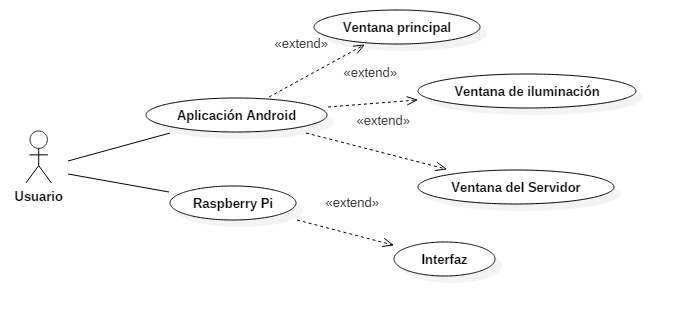
\includegraphics[width=1.2\linewidth]{img/CDUGeneral}
	\caption{Diagrama de casos de uso general.}
	\label{fig:CDUGeneral}
\end{figure}

\subsubsection{Ventana principal}

\begin{enumerate}
	\item Crear estancia.
	\item Modificar nombre.
	\item Eliminar estancia.
	\item Borrar base de datos.
	\item Ir a la ventana del Servidor. 
\end{enumerate}

\subsubsection{Ventana de Iluminación}

\begin{enumerate}
	\item Crear bombilla.
	\item Modificar nombre.
	\item Eliminar bombilla.
	\item Encender bombilla.
	\item Apagar bombilla.
	\item Volver a la ventana principal. 
\end{enumerate}

\subsubsection{Ventana del Servidor}

\begin{enumerate}
	\item Modificar IP
	\item Modificar Puerto.
	\item Conectar al servidor.
	\item Desconectar del servidor.
	\item Volver a la ventana principal.
\end{enumerate}

\subsubsection{Interfaz Raspberry}

\begin{enumerate}
	\item Actualizar IP.
\end{enumerate}

\section{Especificación de requisitos}

En este apartado, una vez hemos visto el diagrama de caso de uso general \ref{fig:CDUGeneral}, vamos a desglosarlo en diagramas de caso de uso más pequeños, \ref{fig:CDUVentanaPrincipal}, \ref{fig:CDUVentanaIluminacion}, \ref{fig:CDUVentanaServidor} y \ref{fig:CDUInterfazPython} que además contienen los requisitos funcionales nombrados en el punto anterior. Además, en las tablas \ref{tabla:CrearEstancia}, \ref{tabla:ModificarNombreEstancia}, \ref{tabla:EliminarEstancia}, \ref{tabla:BorrarBaseDeDatos}, \ref{tabla:ventanaServidor}, \ref{tabla:CrearBombilla}, \ref{tabla:ModificarNombreBombilla}, \ref{tabla:EliminarBombilla}, \ref{tabla:EncenderBombilla}, \ref{tabla:ApagarBombilla}, \ref{tabla:volverVentanaPrincipal}, \ref{tabla:ModificarIP}, \ref{tabla:ModificarPuerto}, \ref{tabla:ConectarAlServidor}, \ref{tabla:DesconectarDelServidor}, \ref{tabla:volverVentanaPrincipalServidor}, \ref{tabla:ActualizarIPPython} se puede ver explicado cada caso de uso con más detalle.

\newpage

\begin{figure}[h!]
	\centering
	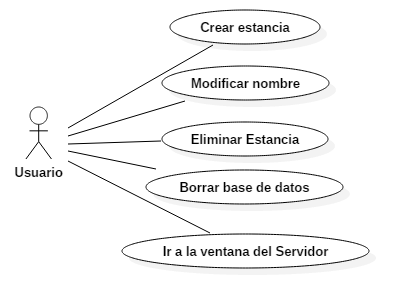
\includegraphics[width=0.7\linewidth]{img/CDUVentanaPrincipal}
	\caption{Funciones que puede realizar el usuario en la ventana principal.}
	\label{fig:CDUVentanaPrincipal}
\end{figure}

\begin{figure}[h!]
	\centering
	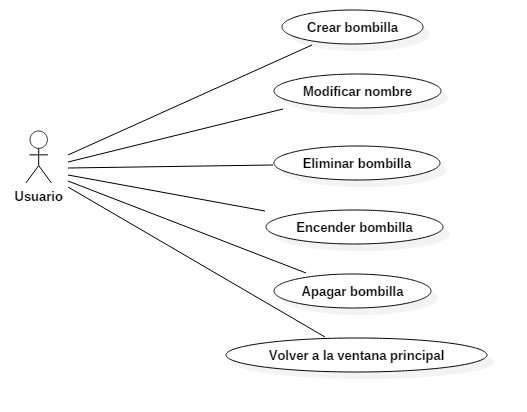
\includegraphics[width=0.9\linewidth]{img/CDUVentanaIluminacion}
	\caption{Funciones que puede realizar el usuario en la ventana de iluminación.}
	\label{fig:CDUVentanaIluminacion}
\end{figure}

\newpage

\begin{figure}[h!]
	\centering
	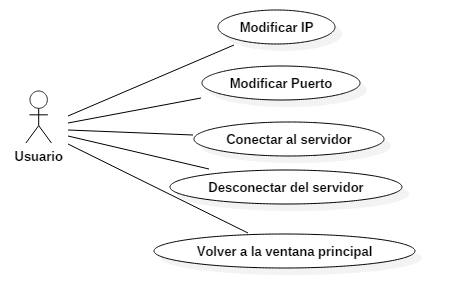
\includegraphics[width=1\linewidth]{img/CDUVentanaServidor}
	\caption{Funciones que puede realizar el usuario en la Ventana del Servidor.}
	\label{fig:CDUVentanaServidor}
\end{figure}

\begin{figure}[h!]
	\centering
	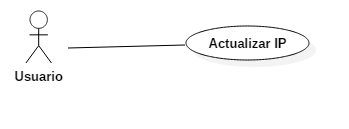
\includegraphics[width=0.8\linewidth]{img/CDUInterfazPython}
	\caption{Funciones que puede realizar el usuario en la interfaz Python.}
	\label{fig:CDUInterfazPython}
\end{figure}

\newpage

\tablaSmallSinColores{Caso de uso ventana principal: \textit{Crear estancia}.}{p{3cm} p{.75cm} p{9.5cm}}{CrearEstancia}{
	\multicolumn{3}{l}{Caso de uso ventana principal: \textit{Crear estancia}.} \\
}
{
	Descripción                            & \multicolumn{2}{p{10.25cm}}{Permite al usuario crear una estancia nueva.} \\\hline
	Requisitos  & \multicolumn{2}{p{10.25cm}}{RF-1} 
	\\\hline
	Precondiciones                         &  \multicolumn{2}{p{10.25cm}}{El usuario debe encontrarse en la ventana principal de la aplicación. \newline Debe estar conectado con el servidor.}   \\\hline
	\multirow{2}{3.5cm}{Secuencia normal}  & Paso & Acción \\\cline{2-3}
	& 1    & El usuario pulsa el botón con símbolo \textbf{+} que se encuentra en la parte superior derecha.
	\\\cline{2-3}
	& 2    & Marca una opción de la lista de estancias en la ventana emergente.
	\\\cline{2-3}
	& 3    & Elige un nombre para esta estancia.
	\\\cline{2-3}
	& 4    & Pulsa sobre el botón \textit{Aceptar} de la ventana emergente.
	\\\hline
	Postcondiciones                        & \multicolumn{2}{p{10.25cm}}{Se ha creado una nueva estancia de ese tipo en la ventana principal.} \\\hline
	Excepciones                        & \multicolumn{2}{p{10.25cm}}{Tratar de crear una estancia sin seleccionar un tipo o escribir un nombre.}\\\hline
	Importancia                            & Alta \\\hline
	Urgencia                               & Alta \\
}

\tablaSmallSinColores{Caso de uso ventana principal: \textit{Modificar nombre}.}{p{3cm} p{.75cm} p{9.5cm}}{ModificarNombreEstancia}{
	\multicolumn{3}{l}{Caso de uso ventana principal: \textit{Modificar nombre}.} \\
}
{
	Descripción                            & \multicolumn{2}{p{10.25cm}}{Permite modificar el nombre de una estancia ya existente.} \\\hline
	Requisitos  & \multicolumn{2}{p{10.25cm}}{RF-2} 
	\\\hline
	Precondiciones                         &  \multicolumn{2}{p{10.25cm}}{El usuario debe encontrarse en la ventana principal de la aplicación. \newline Debe existir al menos una estancia para poder modificar su nombre. \newline Debe estar conectado con el servidor.}   \\\hline
	\multirow{2}{3.5cm}{Secuencia normal}  & Paso & Acción \\\cline{2-3}
	& 1    & Mantener pulsado brevemente sobre la estancia hasta que se muestre el menú contextual.
	\\\cline{2-3}
	& 2    & Seleccionar la opción \textit{Cambiar nombre} del menú contextual.
	\\\cline{2-3}
	& 3    & Escribir el nuevo nombre en la ventana emergente que se nos muestra.
	\\\cline{2-3}
	& 4    & Pulsar sobre el botón \textit{Aceptar} de la ventana emergente.
	\\\hline
	Postcondiciones                        & \multicolumn{2}{p{10.25cm}}{El nombre de la estancia sobre la que estábamos trabajando se ha actualizado.} \\\hline
	Excepciones                        & \multicolumn{2}{p{10.25cm}}{}\\\hline
	Importancia                            & Alta \\\hline
	Urgencia                               & Alta \\
}

\tablaSmallSinColores{Caso de uso ventana principal: \textit{Eliminar estancia}.}{p{3cm} p{.75cm} p{9.5cm}}{EliminarEstancia}{
	\multicolumn{3}{l}{Caso de uso ventana principal: \textit{Eliminar estancia}.} \\
}
{
	Descripción                            & \multicolumn{2}{p{10.25cm}}{Permite eliminar una estancia ya existente.} \\\hline
	Requisitos  & \multicolumn{2}{p{10.25cm}}{RF-3} 
	\\\hline
	Precondiciones                         &  \multicolumn{2}{p{10.25cm}}{El usuario debe encontrarse en la ventana principal de la aplicación. \newline Debe existir al menos una estancia para poder eliminar. \newline Debe estar conectado con el servidor.}   \\\hline
	\multirow{2}{3.5cm}{Secuencia normal}  & Paso & Acción \\\cline{2-3}
	& 1    & Mantener pulsado brevemente sobre la estancia hasta que se muestre el menú contextual.
	\\\cline{2-3}
	& 2    & Seleccionar la opción \textit{Borrar} del menú contextual.
	\\\cline{2-3}
	& 3    & Pulsar sobre el botón \textit{Aceptar} de la ventana emergente de confirmación.
	\\\hline
	Postcondiciones                        & \multicolumn{2}{p{10.25cm}}{La estancia debe desaparecer de la vista actual} \\\hline
	Excepciones                        & \multicolumn{2}{p{10.25cm}}{}\\\hline
	Importancia                            & Alta \\\hline
	Urgencia                               & Alta \\
}

\tablaSmallSinColores{Caso de uso ventana principal: \textit{Borrar base de datos}.}{p{3cm} p{.75cm} p{9.5cm}}{BorrarBaseDeDatos}{
	\multicolumn{3}{l}{Caso de uso ventana principal: \textit{Borrar base de datos}.} \\
}
{
	Descripción                            & \multicolumn{2}{p{10.25cm}}{Permite borrar tanto la base de datos local como la del servidor.} \\\hline
	Requisitos  & \multicolumn{2}{p{10.25cm}}{RF-4} 
	\\\hline
	Precondiciones                         &  \multicolumn{2}{p{10.25cm}}{El usuario debe encontrarse en la ventana principal de la aplicación. \newline Debe estar conectado con el servidor.}   \\\hline
	\multirow{2}{3.5cm}{Secuencia normal}  & Paso & Acción \\\cline{2-3}
	& 1    & Pulsar sobre las tres líneas blancas horizontales de la parte superior izquierda para mostrar el menú desplegable.
	\\\cline{2-3}
	& 2    & Seleccionar la opción \textit{Borrar base de datos} del menú desplegable.
	\\\cline{2-3}
	& 3    & Pulsar sobre el botón \textit{Aceptar} de la ventana emergente de confirmación.
	\\\hline
	Postcondiciones                        & \multicolumn{2}{p{10.25cm}}{Debe borrarse la base de datos local y del servidor.\newline Deben desaparecer todas las estancias que hubiese en la vista.} \\\hline
	Excepciones                        & \multicolumn{2}{p{10.25cm}}{}\\\hline
	Importancia                            & Media \\\hline
	Urgencia                               & Media \\
}

\tablaSmallSinColores{Caso de uso ventana principal: \textit{Ir a la ventana del Servidor}.}{p{3cm} p{.75cm} p{9.5cm}}{ventanaServidor}{
	\multicolumn{3}{l}{Caso de uso ventana principal: \textit{Ir a la ventana del Servidor}.} \\
}
{
	Descripción                            & \multicolumn{2}{p{10.25cm}}{Permite cambiar desde la ventana principal a la ventana del Servidor.} \\\hline
	Requisitos  & \multicolumn{2}{p{10.25cm}}{RF-5} 
	\\\hline
	Precondiciones                         &  \multicolumn{2}{p{10.25cm}}{El usuario debe encontrarse en la ventana principal de la aplicación.}   \\\hline
	\multirow{2}{3.5cm}{Secuencia normal}  & Paso & Acción \\\cline{2-3}
	& 1    & Pulsar sobre las tres líneas blancas horizontales de la parte superior izquierda para mostrar el menú desplegable.
	\\\cline{2-3}
	& 2    & Seleccionar la opción \textit{Servidor} del menú desplegable.
	\\\hline
	Postcondiciones                        & \multicolumn{2}{p{10.25cm}}{Deberá encontrarse en la ventana del Servidor} \\\hline
	Excepciones                        & \multicolumn{2}{p{10.25cm}}{}\\\hline
	Importancia                            & Alta \\\hline
	Urgencia                               & Media \\
}

\tablaSmallSinColores{Caso de uso ventana de iluminación: \textit{Crear bombilla}.}{p{3cm} p{.75cm} p{9.5cm}}{CrearBombilla}{
	\multicolumn{3}{l}{Caso de uso ventana de iluminación: \textit{Crear bombilla}.} \\
}
{
	Descripción                            & \multicolumn{2}{p{10.25cm}}{Permite al usuario crear una bombilla nueva.} \\\hline
	Requisitos  & \multicolumn{2}{p{10.25cm}}{RF-1} 
	\\\hline
	Precondiciones                         &  \multicolumn{2}{p{10.25cm}}{El usuario debe encontrarse en la ventana de iluminación de la aplicación. \newline Debe estar conectado con el servidor.}   \\\hline
	\multirow{2}{3.5cm}{Secuencia normal}  & Paso & Acción \\\cline{2-3}
	& 1    & El usuario pulsa el botón con símbolo \textbf{+} que se encuentra en la parte superior derecha.
	\\\cline{2-3}
	& 2    & Marca la única opción existente en la ventana emergente.
	\\\cline{2-3}
	& 3    & Elige un nombre para esta bombilla.
	\\\cline{2-3}
	& 4    & Pulsa sobre el botón \textit{Aceptar} de la ventana emergente.
	\\\hline
	Postcondiciones                        & \multicolumn{2}{p{10.25cm}}{Se ha creado una nueva bombilla en la ventana de iluminación.} \\\hline
	Excepciones                        & \multicolumn{2}{p{10.25cm}}{Tratar de crear una bombilla sin seleccionarla en la lista o escribir un nombre.}\\\hline
	Importancia                            & Alta \\\hline
	Urgencia                               & Alta \\
}

\tablaSmallSinColores{Caso de uso ventana de iluminación: \textit{Modificar nombre}.}{p{3cm} p{.75cm} p{9.5cm}}{ModificarNombreBombilla}{
	\multicolumn{3}{l}{Caso de uso ventana de iluminación: \textit{Modificar nombre}.} \\
}
{
	Descripción                            & \multicolumn{2}{p{10.25cm}}{Permite modificar el nombre de una bombilla ya existente.} \\\hline
	Requisitos  & \multicolumn{2}{p{10.25cm}}{RF-2} 
	\\\hline
	Precondiciones                         &  \multicolumn{2}{p{10.25cm}}{El usuario debe encontrarse en la ventana de iluminación de la aplicación. \newline Debe existir al menos una bombilla para poder modificar su nombre. \newline Debe estar conectado con el servidor.}   \\\hline
	\multirow{2}{3.5cm}{Secuencia normal}  & Paso & Acción \\\cline{2-3}
	& 1    & Mantener pulsado brevemente sobre la bombilla hasta que se muestre el menú contextual.
	\\\cline{2-3}
	& 2    & Seleccionar la opción \textit{Cambiar nombre} del menú contextual.
	\\\cline{2-3}
	& 3    & Escribir el nuevo nombre en la ventana emergente que se nos muestra.
	\\\cline{2-3}
	& 4    & Pulsar sobre el botón \textit{Aceptar} de la ventana emergente.
	\\\hline
	Postcondiciones                        & \multicolumn{2}{p{10.25cm}}{El nombre de la bombilla sobre la que estábamos trabajando se ha actualizado.} \\\hline
	Excepciones                        & \multicolumn{2}{p{10.25cm}}{}\\\hline
	Importancia                            & Alta \\\hline
	Urgencia                               & Alta \\
}

\tablaSmallSinColores{Caso de uso ventana de iluminación: \textit{Eliminar bombilla}.}{p{3cm} p{.75cm} p{9.5cm}}{EliminarBombilla}{
	\multicolumn{3}{l}{Caso de uso ventana de iluminación: \textit{Eliminar bombilla}.} \\
}
{
	Descripción                            & \multicolumn{2}{p{10.25cm}}{Permite eliminar una bombilla ya existente.} \\\hline
	Requisitos  & \multicolumn{2}{p{10.25cm}}{RF-3} 
	\\\hline
	Precondiciones                         &  \multicolumn{2}{p{10.25cm}}{El usuario debe encontrarse en la ventana de iluminación de la aplicación. \newline Debe existir al menos una bombilla para poder eliminar. \newline Debe estar conectado con el servidor.}   \\\hline
	\multirow{2}{3.5cm}{Secuencia normal}  & Paso & Acción \\\cline{2-3}
	& 1    & Mantener pulsado brevemente sobre la bombilla hasta que se muestre el menú contextual.
	\\\cline{2-3}
	& 2    & Seleccionar la opción \textit{Borrar} del menú contextual.
	\\\cline{2-3}
	& 3    & Pulsar sobre el botón \textit{Aceptar} de la ventana emergente de confirmación.
	\\\hline
	Postcondiciones                        & \multicolumn{2}{p{10.25cm}}{La bombilla debe desaparecer de la vista actual.} \\\hline
	Excepciones                        & \multicolumn{2}{p{10.25cm}}{}\\\hline
	Importancia                            & Alta \\\hline
	Urgencia                               & Alta \\
}

\tablaSmallSinColores{Caso de uso ventana de iluminación: \textit{Encender bombilla}.}{p{3cm} p{.75cm} p{9.5cm}}{EncenderBombilla}{
	\multicolumn{3}{l}{Caso de uso ventana de iluminación: \textit{Encender bombilla}.} \\
}
{
	Descripción                            & \multicolumn{2}{p{10.25cm}}{Permite cambiar el estado de la bombilla a \textit{Encendida}} \\\hline
	Requisitos  & \multicolumn{2}{p{10.25cm}}{RF-4} 
	\\\hline
	Precondiciones                         &  \multicolumn{2}{p{10.25cm}}{El usuario debe encontrarse en la ventana de iluminación de la aplicación. \newline Debe existir al menos una bombilla para poder encenderla. \newline El interruptor deben estar apagado. \newline Debe estar conectado con el servidor.}   \\\hline
	\multirow{2}{3.5cm}{Secuencia normal}  & Paso & Acción \\\cline{2-3}
	& 1    & Pulsar el interruptor de la bombilla para cambiar su estado y encenderla.
	\\\hline
	Postcondiciones                        & \multicolumn{2}{p{10.25cm}}{La bombilla debe encenderse, cambiando su imagen y su estado.} \\\hline
	Excepciones                        & \multicolumn{2}{p{10.25cm}}{}\\\hline
	Importancia                            & Alta \\\hline
	Urgencia                               & Alta \\
}

\tablaSmallSinColores{Caso de uso ventana de iluminación: \textit{Apagar bombilla}.}{p{3cm} p{.75cm} p{9.5cm}}{ApagarBombilla}{
	\multicolumn{3}{l}{Caso de uso ventana de iluminación: \textit{Apagar bombilla}.} \\
}
{
	Descripción                            & \multicolumn{2}{p{10.25cm}}{Permite cambiar el estado de la bombilla a \textit{Apagada}} \\\hline
	Requisitos  & \multicolumn{2}{p{10.25cm}}{RF-5}
	\\\hline
	Precondiciones                         &  \multicolumn{2}{p{10.25cm}}{El usuario debe encontrarse en la ventana de iluminación de la aplicación. \newline Debe existir al menos una bombilla para poder apagarla. \newline El interruptor deben estar encendido. \newline Debe estar conectado con el servidor.}   \\\hline
	\multirow{2}{3.5cm}{Secuencia normal}  & Paso & Acción \\\cline{2-3}
	& 1    & Pulsar el interruptor de la bombilla para cambiar su estado y apagarla.
	\\\hline
	Postcondiciones                        & \multicolumn{2}{p{10.25cm}}{La bombilla debe apagarse, cambiando su imagen y su estado.} \\\hline
	Excepciones                        & \multicolumn{2}{p{10.25cm}}{}\\\hline
	Importancia                            & Alta \\\hline
	Urgencia                               & Alta \\
}

\tablaSmallSinColores{Caso de uso ventana de iluminación: \textit{Volver a la ventana principal}.}{p{3cm} p{.75cm} p{9.5cm}}{volverVentanaPrincipal}{
	\multicolumn{3}{l}{Caso de uso ventana de iluminación: \textit{Volver a la ventana principal}.} \\
}
{
	Descripción                            & \multicolumn{2}{p{10.25cm}}{Permite ir desde la ventana de iluminación a la ventana principal.} \\\hline
	Requisitos  & \multicolumn{2}{p{10.25cm}}{RF-6} 
	\\\hline
	Precondiciones                         &  \multicolumn{2}{p{10.25cm}}{El usuario debe encontrarse en la ventana de iluminación de la aplicación.}   \\\hline
	\multirow{2}{3.5cm}{Secuencia normal}  & Paso & Acción \\\cline{2-3}
	& 1    & Pulsar sobre la flecha que se encuentra en la parte superior izquierda.
	\\\hline
	Postcondiciones                        & \multicolumn{2}{p{10.25cm}}{Nos encontramos en la ventana principal.} \\\hline
	Excepciones                        & \multicolumn{2}{p{10.25cm}}{}\\\hline
	Importancia                            & Media \\\hline
	Urgencia                               & Media \\
}



\tablaSmallSinColores{Caso de uso ventana del Servidor: \textit{Modificar IP}.}{p{3cm} p{.75cm} p{9.5cm}}{ModificarIP}{
	\multicolumn{3}{l}{Caso de uso ventana del Servidor: \textit{Modificar IP}.} \\
}
{
	Descripción                            & \multicolumn{2}{p{10.25cm}}{Actualiza el valor asignado a la IP del servidor.} \\\hline
	Requisitos  & \multicolumn{2}{p{10.25cm}}{RF-1} 
	\\\hline
	Precondiciones                         &  \multicolumn{2}{p{10.25cm}}{El usuario debe encontrarse en la ventana de servidor de la aplicación.}   \\\hline
	\multirow{2}{3.5cm}{Secuencia normal}  & Paso & Acción \\\cline{2-3}
	& 1    & Pulsar sobre el campo de texto de la IP.
	\\\cline{2-3}
	& 2    & Escribir la nueva IP que se quiera utilizar.
	\\\cline{2-3}
	& 3    & Pulsar sobre el botón \textit{Actualizar}.
	\\\hline
	Postcondiciones                        & \multicolumn{2}{p{10.25cm}}{La IP ha sido guardada en la base de datos.} \\\hline
	Excepciones                        & \multicolumn{2}{p{10.25cm}}{}\\\hline
	Importancia                            & Alta \\\hline
	Urgencia                               & Alta \\
}

\tablaSmallSinColores{Caso de uso ventana del Servidor: \textit{Modificar Puerto}.}{p{3cm} p{.75cm} p{9.5cm}}{ModificarPuerto}{
	\multicolumn{3}{l}{Caso de uso ventana del Servidor: \textit{Modificar Puerto}.} \\
}
{
	Descripción                            & \multicolumn{2}{p{10.25cm}}{Actualiza el valor asignado a la IP del servidor.} \\\hline
	Requisitos  & \multicolumn{2}{p{10.25cm}}{RF-2} 
	\\\hline
	Precondiciones                         &  \multicolumn{2}{p{10.25cm}}{El usuario debe encontrarse en la ventana de servidor de la aplicación.}   \\\hline
	\multirow{2}{3.5cm}{Secuencia normal}  & Paso & Acción \\\cline{2-3}
	& 1    & Pulsar sobre el campo de texto del Puerto.
	\\\cline{2-3}
	& 2    & Escribir el nuevo Puerto que se quiera utilizar.
	\\\cline{2-3}
	& 3    & Pulsar sobre el botón \textit{Actualizar}.
	\\\hline
	Postcondiciones                        & \multicolumn{2}{p{10.25cm}}{El Puerto se guarda en la base de datos.} \\\hline
	Excepciones                        & \multicolumn{2}{p{10.25cm}}{}\\\hline
	Importancia                            & Alta \\\hline
	Urgencia                               & Alta \\
}

\tablaSmallSinColores{Caso de uso ventana del Servidor: \textit{Conectar al servidor}.}{p{3cm} p{.75cm} p{9.5cm}}{ConectarAlServidor}{
	\multicolumn{3}{l}{Caso de uso ventana del Servidor: \textit{Conectar al servidor}.} \\
}
{
	Descripción                            & \multicolumn{2}{p{10.25cm}}{Crea una conexión con el Servidor.} \\\hline
	Requisitos  & \multicolumn{2}{p{10.25cm}}{RF-3} 
	\\\hline
	Precondiciones                         &  \multicolumn{2}{p{10.25cm}}{El usuario debe encontrarse en la ventana de servidor de la aplicación.\newline El campo IP debe contener una IP válida. \newline El campo Puerto debe contener un puerto válido.}   \\\hline
	\multirow{2}{3.5cm}{Secuencia normal}  & Paso & Acción \\\cline{2-3}
	& 1    & Pulsar el botón \textit{Conectar}.
	\\\hline
	Postcondiciones                        & \multicolumn{2}{p{10.25cm}}{El estado del servidor pasa a \textit{Conectado}.} \\\hline
	Excepciones                        & \multicolumn{2}{p{10.25cm}}{}\\\hline
	Importancia                            & Alta \\\hline
	Urgencia                               & Alta \\
}

\tablaSmallSinColores{Caso de uso ventana del Servidor: \textit{Desconectar del servidor}.}{p{3cm} p{.75cm} p{9.5cm}}{DesconectarDelServidor}{
	\multicolumn{3}{l}{Caso de uso ventana de servidor: \textit{Desconectar del servidor}.} \\
}
{
	Descripción                            & \multicolumn{2}{p{10.25cm}}{Cierra una conexión existente con el Servidor.} \\\hline
	Requisitos  & \multicolumn{2}{p{10.25cm}}{RF-4} 
	\\\hline
	Precondiciones                         &  \multicolumn{2}{p{10.25cm}}{El usuario debe encontrarse en la ventana del Servidor de la aplicación.\newline Debe existir una conexión con el Servidor actualmente.}   \\\hline
	\multirow{2}{3.5cm}{Secuencia normal}  & Paso & Acción \\\cline{2-3}
	& 1    & Pulsar el botón \textit{Desconectar}.
	\\\hline
	Postcondiciones                        & \multicolumn{2}{p{10.25cm}}{El estado del servidor pasa a \textit{Desconectado}.} \\\hline
	Excepciones                        & \multicolumn{2}{p{10.25cm}}{}\\\hline
	Importancia                            & Alta \\\hline
	Urgencia                               & Alta \\
}

\tablaSmallSinColores{Caso de uso ventana del Servidor: \textit{Volver a la ventana principal}.}{p{3cm} p{.75cm} p{9.5cm}}{volverVentanaPrincipalServidor}{
	\multicolumn{3}{l}{Caso de uso ventana del Servidor: \textit{Volver a la ventana principal}.} \\
}
{
	Descripción                            & \multicolumn{2}{p{10.25cm}}{Permite ir desde la ventana del Servidor a la ventana principal.} \\\hline
	Requisitos  & \multicolumn{2}{p{10.25cm}}{RF-5} 
	\\\hline
	Precondiciones                         &  \multicolumn{2}{p{10.25cm}}{El usuario debe encontrarse en la ventana del Servidor de la aplicación.}   \\\hline
	\multirow{2}{3.5cm}{Secuencia normal}  & Paso & Acción \\\cline{2-3}
	& 1    & Pulsar sobre la flecha que se encuentra en la parte superior izquierda.
	\\\hline
	Postcondiciones                        & \multicolumn{2}{p{10.25cm}}{Nos encontramos en la ventana principal} \\\hline
	Excepciones                        & \multicolumn{2}{p{10.25cm}}{}\\\hline
	Importancia                            & Media \\\hline
	Urgencia                               & Media \\
}

\tablaSmallSinColores{Caso de uso Interfaz Python: \textit{Actualizar IP}.}{p{3cm} p{.75cm} p{9.5cm}}{ActualizarIPPython}{
	\multicolumn{3}{l}{Caso de uso Interfaz Python: \textit{Actualizar IP}.} \\
}                                                        
{
	Descripción                            & \multicolumn{2}{p{10.25cm}}{Permite introducir una IP nueva.} \\\hline
	Requisitos  & \multicolumn{2}{p{10.25cm}}{RF-1} 
	\\\hline
	Precondiciones                         &  \multicolumn{2}{p{10.25cm}}{El usuario debe encontrarse en la Interfaz Python del Servidor tras arrancar el Servidor.\newline La IP debe estar vacía o incorrecta.}   \\\hline
	\multirow{2}{3.5cm}{Secuencia normal}  & Paso & Acción \\\cline{2-3}
	& 1    & En el error que se muestre, pulsar el botón \textit{Aceptar}.
	\\\cline{2-3}
	& 2    & En la nueva ventana que se abrirá, escribir la nueva IP en el cuadro de texto correspondiente.
	\\\cline{2-3}
	& 3    & Pulsar el botón \textit{Actualizar}.
	\\\hline
	Postcondiciones                        & \multicolumn{2}{p{10.25cm}}{El socket estará escuchando correctamente en esa IP.} \\\hline
	Excepciones                        & \multicolumn{2}{p{10.25cm}}{}\\\hline
	Importancia                            & Alta \\\hline
	Urgencia                               & Alta \\
}
\apendice{Especificación de diseño}

\section{Introducción}

En este apéndice vamos a hablar sobre los diferentes aspectos de diseño.

\section{Diseño de datos}

En este proyecto se trabaja con muchos datos, pero la mayoría de ellos son del mismo tipo. Se trabaja con gran cantidad de Strings o cadenas de caracteres. La lógica de trabajar con cadenas de caracteres frente a otros tipos de datos radica en la facilidad para ser leídos a través de un \textit{buffer} o incluso de ser tratados. Además, hay que tener en cuenta que ciertos tipos de datos no pueden ser almacenados o enviados. Por ejemplo, en nuestra base de datos querríamos almacenar el estado de las luces mediante una variable de tipo \verb|boolean|, pero nuestra base de datos \textbf{Sqlite} no permite alamcenarlos. En su defecto, el estado de las luces ha tenido que ser guardado mediante una variable de tipo \verb|Integer| que podrá contener los valores \textit{0} o \textit{1}.

En nuestra base de datos, ya sea en la parte de Raspberry Pi o de Android, solo almacenaremos cadenas de caracteres (\verb|Strings|) o números (\verb|Integer|). A través de la conexión entre clientes y servidor solo se manda cadenas de caracteres a través de un \textit{buffer} para realizar cambios en cualquiera de las partes. Solamente se ha hablado de estos dos tipos de datos porque son los dos únicos tipos que o se almacenan para su tratamiento o son tratados en el momento.

\section{Diseño procedimental}

\begin{figure}[h!]
	\centering
	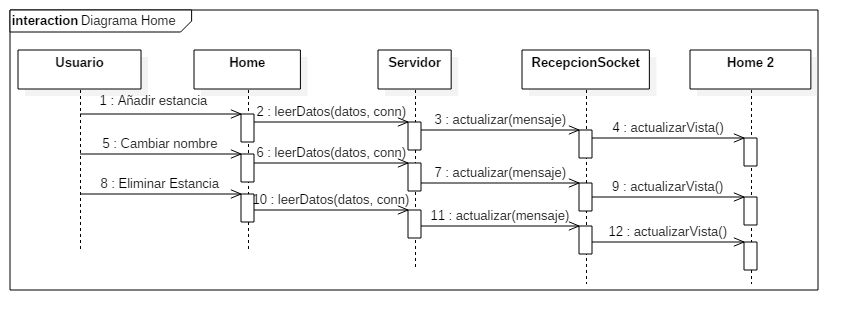
\includegraphics[width=1.2\linewidth]{img/DiagramaHome}
	\caption{Diagrama de acciones sobre una estancia en la clase \textbf{Home}.}
	\label{fig:DiagramaHome}
\end{figure}

\begin{figure}[h!]
	\centering
	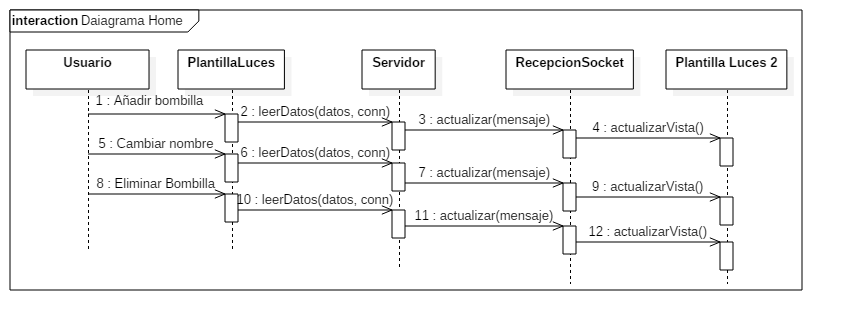
\includegraphics[width=1.2\linewidth]{img/DiagramaPlantillaLuces}
	\caption{Diagrama de acciones sobre una bombilla en la clase \textbf{PlantillaLuces}.}
	\label{fig:DiagramaPlantillaLuces}
\end{figure}

\section{Diseño arquitectónico}

En este apartado hablaremos del diseño arquitectónico de ambas partes del proyecto.

\subsection{Raspberry Pi}

En esta parte del proyecto no existen paquetes que agrupen los ficheros y los archivos se encuentran en la raíz del proyecto. Vamos a hablar brevemente de los métodos y características de estos ficheros.

\subsubsection{Servidor.py}

En este fichero se encuentra la implementación de la clase \textit{Servidor} que contiene los siguientes métodos.

\begin{itemize}
	\item \verb|__init__(self)|: se encarga de inicializar las variables, iniciar la interfaz y arrancar el servidor en un hilo independiente.
	\item \verb|iniciarInterfaz(self)|: se encarga de inicializar todas la variables y estructuras de la interfaz y arrancarla.
	\item \verb|centrarVentana(self, ventana, widht, height)|: centra la ventana pasada por parámetro con un tamaño igual a \textit{widht} y \textit{height}.
	\item \verb|agregarIp(self)|: se encarga de mostrar una nueva ventana desde la que poder actualizar la IP.
	\item \verb|actualizarIp(self)|: se encarga de recoger el valor de la IP que se ha introducido en la ventana creada por \verb|agregarIp(self)|.
	\item \verb|leerDatos(self, datos, conn)|: se encarga de interpretar todos los mensajes que llegan al servidor y actuar en medida de lo que se ha leído.
	\item \verb|clienteThread(self, conn)|: se encarga de crear un nuevo hilo independiente para cada conexión de un cliente con el servidor.
	\item \verb|iniciarServidor(self)|: se encarga de inicializar todas las variables y estructuras del servidor y arrancarlo.
	\item \verb|main()|: se encarga de realizar la ejecución principal del archivo.
\end{itemize}

\subsubsection{Database.py}

En este fichero se encuentra la implementación de la clase \textit{Database} que contiene los siguiente métodos

\begin{itemize}
	\item \verb|__init__(self)|: se encarga de crear las tablas de la base de datos si no estuviesen ya creadas.
	\item \verb|insertarEstancia(self, id, nombre)|: se encarga de insertar una nueva estancia en la base de datos.
	\item \verb|insertarElemento(self, estancia, nombre, estado)|: se encarga de insertar un nuevo elemento en la base de datos.
	\item \verb|actualizarEstancia(self, nombreViejo, nombreNuevo)|: se encarga de actualizar el nombre de una estancia de la base de datos.
	\item \verb|actualizarElemento(self, estancia, nombreViejo, nombreNuevo)|: se encarga de actualizar nombre de un elemento de una estancia de la base de datos.
	\item \verb|actualizarEstado(self, estancia, nombre, estado)|: se encarga de actualizar el estado de un elemento de una estancia de la base de datos.
	\item \verb|actualizarIP(self, ip)|: se encarga de actualizar la IP de la base de datos.
	\item \verb|eliminarEstancia(self, estancia)|: se encarga de eliminar una estancia de la base de datos.
	\item \verb|eliminarElemento(self, estancia, index)|: se encarga de eliminar un elemento de una estancia de la base de datos.
	\item \verb|recuperarEstancia(self, index)|: se encarga de devolver una estancia de la base de datos.
	\item \verb|recuperarElemento(self, estancia, index)|: se encarga de devolver un elemento de la base de datos.
	\item \verb|recuperarIp(self)|: se encarga de devolver la ip almacenada en la base de datos.
	\item \verb|numeroEstancias(self)|: se encarga de devolver el número de estancias en la base de datos.
	\item \verb|numeroElementos(self, estancia)|: se encarga de devolver el número de elementos de una estancia de la base de datos.
	\item \verb|cerrarBD(self)|: se encarga de cerrar la conexión con la base de datos.
	\item \verb|borrarBD(self)|: se encarga de borrar todas las tablas de la base de datos.
\end{itemize}

\subsubsection{Aplicación Android}

En esta parte del proyecto no existen paquetes para diferenciar unas clases de otras, todas se encuentran en el directorio \textbf{Simulador Domotica Raspberry/app android/app/src/main/java/mario/app android}. La función de cada una de las clases la podemos encontrar en la sección \ref{sec:explicacionAndroid}. Aquí simplemente vamos a visualizar el diagrama de clases de cada uno de los ficheros \textit{.java} de ese directorio.

\begin{enumerate}
	\item \verb|BDLocal|: \ref{fig:BDLocal}
	\begin{figure}[h!]
		\centering
		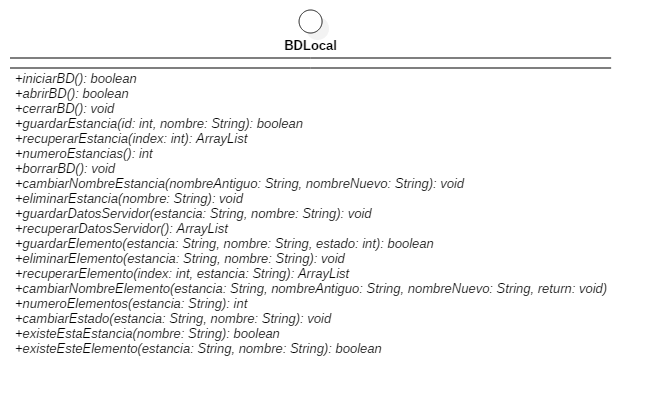
\includegraphics[width=1.1\linewidth]{img/BDLocal}
		\caption{Diagrama de la clase \textbf{BDLocal}.}
		\label{fig:BDLocal}
	\end{figure}
	\item \verb|SQLite|: \ref{fig:SQLite}
	\begin{figure}[h!]
		\centering
		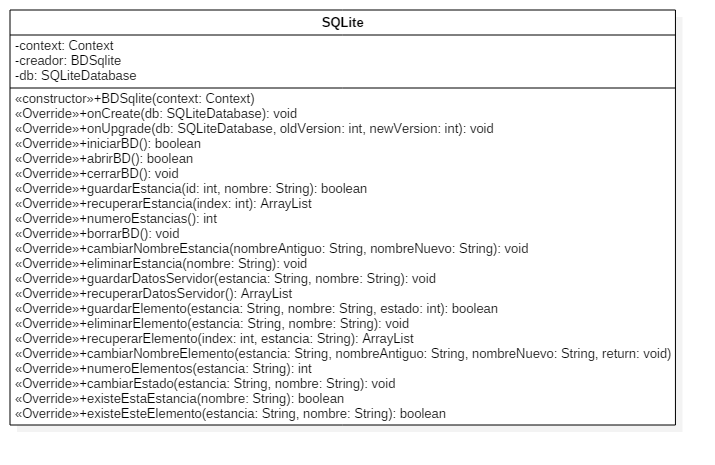
\includegraphics[width=1.1\linewidth]{img/SQLite}
		\caption{Diagrama de la clase \textbf{SQLite}.}
		\label{fig:SQLite}
	\end{figure}
	\item \verb|Conexion|: \ref{fig:Conexion}
	\begin{figure}[h!]
		\centering
		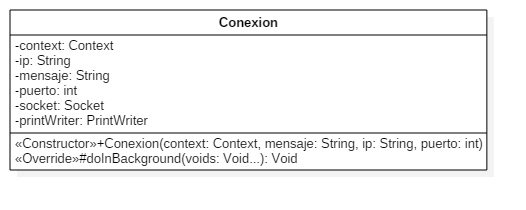
\includegraphics[width=1.1\linewidth]{img/Conexion}
		\caption{Diagrama de la clase \textbf{Conexion}.}
		\label{fig:Conexion}
	\end{figure}
	\item \verb|CustomAdapterEstancia|: \ref{fig:CustomAdapterEstancia}
	\begin{figure}[h!]
		\centering
		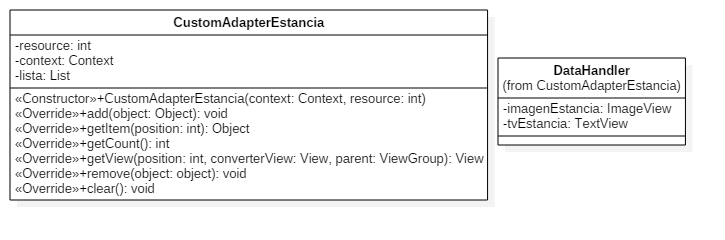
\includegraphics[width=1.2\linewidth]{img/CustomAdapterEstancia}
		\caption{Diagrama de la clase \textbf{CustomAdapterEstancia}.}
		\label{fig:CustomAdapterEstancia}
	\end{figure}
	\item \verb|CustomAdapterLuz|: \ref{fig:CustomAdapterLuz}
	\begin{figure}[h!]
		\centering
		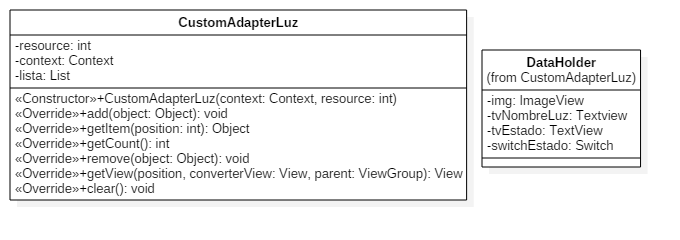
\includegraphics[width=1.3\linewidth]{img/CustomAdapterLuz}
		\caption{Diagrama de la clase \textbf{CustomAdapterLuz}.}
		\label{fig:CustomAdapterLuz}
	\end{figure}
	\item \verb|Habitacion|: \ref{fig:Habitacion}
	\begin{figure}[h!]
		\centering
		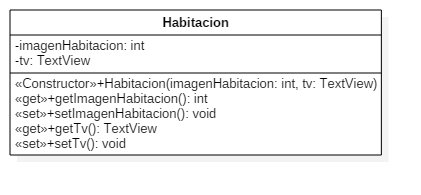
\includegraphics[width=1\linewidth]{img/Habitacion}
		\caption{Diagrama de la clase \textbf{Habitacion}.}
		\label{fig:Habitacion}
	\end{figure}
	\item \verb|Home|: \ref{fig:Home}
	\begin{figure}[h!]
		\centering
		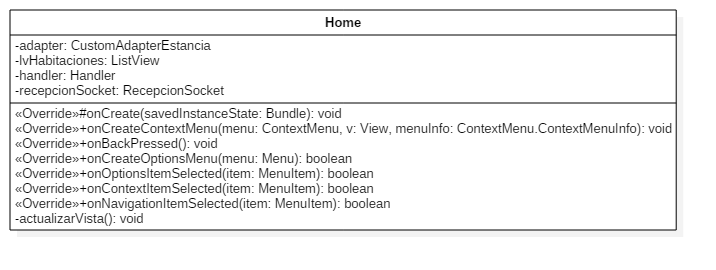
\includegraphics[width=1.2\linewidth]{img/Home}
		\caption{Diagrama de la clase \textbf{Home}.}
		\label{fig:Home}
	\end{figure}
	\item \verb|Luz|: \ref{fig:Luz}
	\begin{figure}[h!]
		\centering
		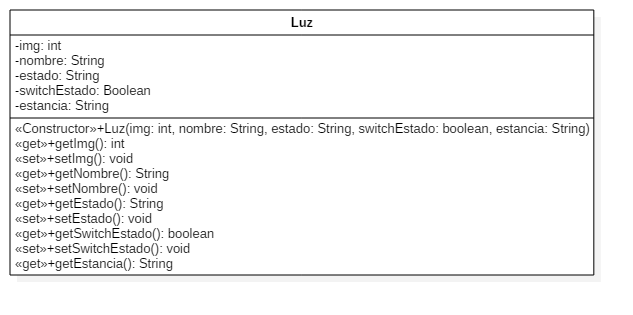
\includegraphics[width=1.2\linewidth]{img/Luz}
		\caption{Diagrama de la clase \textbf{Luz}.}
		\label{fig:Luz}
	\end{figure}
	\item \verb|PlantillaLuces|: \ref{fig:PlantillaLuces}
	\begin{figure}[h!]
		\centering
		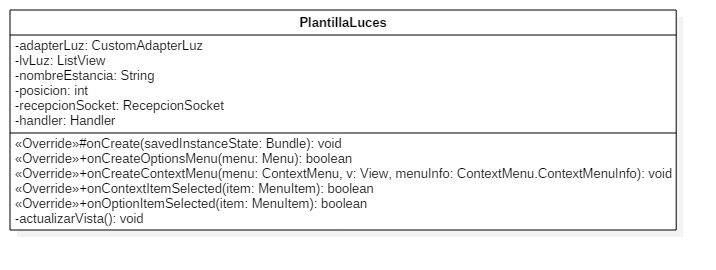
\includegraphics[width=1.3\linewidth]{img/PlantillaLuces}
		\caption{Diagrama de la clase \textbf{PlantillaLuces}.}
		\label{fig:PlantillaLuces}
	\end{figure}
	\item \verb|RecepcionSocket|: \ref{fig:RecepcionSocket}
	\begin{figure}[h!]
		\centering
		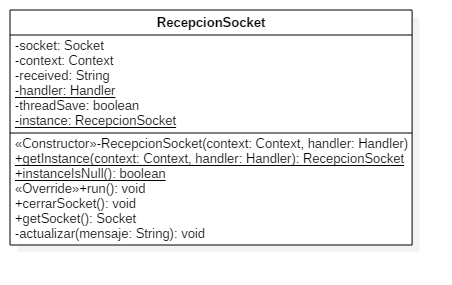
\includegraphics[width=1\linewidth]{img/RecepcionSocket}
		\caption{Diagrama de la clase \textbf{RecepcionSocket}.}
		\label{fig:RecepcionSocket}
	\end{figure}
	\item \verb|Servidor|: \ref{fig:DiagramaServidor}
	\begin{figure}[h!]
		\centering
		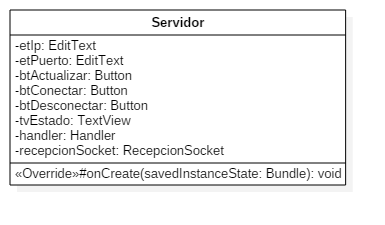
\includegraphics[width=0.9\linewidth]{img/DiagramaServidor}
		\caption{Diagrama de la clase \textbf{Servidor}.}
		\label{fig:DiagramaServidor}
	\end{figure}
\end{enumerate}
\apendice{Documentación técnica de programación}

\section{Introducción}

En este apéndice voy a tratar de explicar todos los detalles técnicos necesarios para que las personas que desean trabajar con este proyecto o incluso continuarlo puedan hacerlo de manera sencilla.

\section{Estructura de directorios}

La siguiente estructura de directorios es la utilizada para la realización del proyecto y se puede encontrar en el siguiente repositorio \url{https://github.com/MJ0T4/Simulador_Domotica_Raspberry}.

\begin{itemize}
	\item \textbf{'/':} directorio raíz del proyecto. En el se encuentra el fichero \textit{README.md} y los siguientes directorios:
	\begin{itemize}
		\item \textbf{apk:} contiene la apk para realizar la instalación de la aplicación
		\item \textbf{app android:} contiene todo el proyecto referente a la parte de \textit{Android} con Android Studio.
		\begin{itemize}
			\item \textbf{app:} contiene el código fuente del proyecto.
			\begin{itemize}
				\item \textbf{src:} contiene el código fuente del proyecto.
				\begin{enumerate}
					\item \textbf{androidTest/java/mario/app android:} contiene los test instrumentales.
					\item \textbf{main}: contiene todas las clases java y todos los recursos del proyecto.
					\item \textbf{test/java/mario/app android:} contiene los test unitarios.
				\end{enumerate}
			\end{itemize}
		\end{itemize}
		\item \textbf{diseño:} contiene el archivo \textit{diseño.mdj} que contiene a su vez todos los diagramas realizado para este proyecto.
		\item \textbf{doc:} contiene la documentación del proyecto.
		\begin{itemize}
			\item \textbf{img:} contiene todas las imágenes utilizadas para la documentación de la memoria y anexos.
			\item \textbf{tex:} contiene cada uno de los ficheros correspondientes a la memoria y anexos.
		\end{itemize}
		\item \textbf{servidor raspberry:} contiene todo el proyecto referente a la parte de \textit{Python 3} con Jetbrains PyCharms.
		\begin{itemize}
			\item \textbf{imagenes:} contiene todas la imágenes utilizadas por la interfaz.
		\end{itemize}
	\end{itemize}
\end{itemize}

\section{Manual del programador}

En este apartado voy a hacer una breve explicación técnica del funcionamiento del proyecto.

\subsection{Raspberry Pi}

En la Raspberry Pi ejecutaremos el código desarrollado en Python 3. Dentro del directorio del proyecto de Python tenemos dos ficheros fundamentales.

\begin{itemize}
	\item El fichero \verb|Servidor.py| contiene toda la lógica de la interfaz y el servidor.
	\item El fichero \verb|Database.py| contiene todos los métodos que permiten realizar cambios en la base de datos.
\end{itemize}

Dentro del fichero \verb|Servidor.py| solo se encuentra una clase que controla todo. Dentro de ella existen métodos para la creación de la interfaz y su tratamiento y métodos para la inicialización del servidor y el tratamiento de mensajes. El hilo de ejecución de ambos se realiza a la vez en la llamada a la clase, pero cada uno tiene su hilo independiente.

\subsection{Aplicación Android}\label{sec:explicacionAndroid}

En este apartado sobre hablaré brevemente sobre los ficheros .java que se encuentran en el directorio \textbf{Simulador Domotica Raspberry/app android/app/src/main/java/mario/app android}. Dentro de este directorio nos encontramos con los siguientes ficheros.

\begin{itemize}
	\item \verb|BDLocal.java|: interfaz creada para declarar, pero no implementar, los métodos que se usarán para realizar cambios en la base de datos.
	\item \verb|BDSqlite.java|: implementa la interfaz \verb|BDLocal.java| y desarrolla los métodos declarados por ella.
	\item \verb|Conexion.java|: implementa una tarea asíncrona para mandar cambios al servidor.
	\item \verb|CustomAdapterEstancia.java|: adaptador personalizado para representar las filas de estancias en una \textit{ListView}.
	\item \verb|CustomAdapterLuz.java|: adaptador personalizado para representar las filas de bombillas en una \textit{ListView}.
	\item \verb|Habitacion.java|: implementa los elementos que irán en cada fila del adaptador \verb|CustomAdapterEstancia.java|.
	\item \verb|Home.java|: implementa la ventana principal donde se representarán las estancias de nuestra vivienda.
	\item \verb|Luz.java|: implementa los elementos que irán en cada fila del adaptador \verb|CustomAdapterLuz.java|.
	\item \verb|PlantillaLuces.java|: implementa la \textit{Activity} en la que se mostrarán las bombillas de una estancia.
	\item \verb|RecepcionSocket.java|: implementa la escucha de mensajes del servidor en un \verb|Thread| implementado la interfaz \verb|Runnable|.
	\item \verb|Servidor.java|: implementa la modificación de datos del servidor, su conexión y desconexión.
\end{itemize}

\section{Compilación, instalación y ejecución del proyecto}

Para comenzar con la compilación del proyecto es necesario descargarlo a través de \textit{GitHub} \url{https://github.com/MJ0T4/Simulador_Domotica_Raspberry}. Una vez tenemos el proyecto descomprimido comenzamos a trabajar con él.

Para realizar la compilación del proyecto Android, tendremos que instalar previamente la herramienta de desarrollo \textbf{Android Studio}. Para ello, podemos descargar el ejecutable desde el siguiente enlace:

\url{https://developer.android.com/studio/}

Una vez descargado e instalado, lo ejecutamos. Dentro de la ventana principal nos digirimos al menú superior de opciones. En el seguiremos los siguientes pasos:
\begin{enumerate}
	\item Pulsar sobre la opción \verb|File| del menú de opciones.
	\item Pulsar sobre la opción \verb|New| del menú que se ha desplegado.
	\item Pulsar sobre la opción \verb|Import project| del menú que se ha desplegado nuevamente.
	\item Se abrirá un explorador de archivos en el que debemos buscar el directorio \verb|app_android| del proyecto que hemos descargado.
	\item Una vez seleccionado lo cargamos y ya tendremos el proyecto en nuestro Android Studio.
\end{enumerate}

Con el proyecto ya cargado en la herramienta Android Studio solo debemos pulsar sobre el icono de un martillo verde y el proyecto comenzará a compilarse.

\begin{figure}[h!]
	\centering
	
\includegraphics[width=0.4\linewidth]{img/martillo}
	\caption{Icono para la compilación del proyecto.}
	\label{fig:martillo}
\end{figure}

La ejecución del proyecto es posible realizarla sobre un emulador virtual de Android que viene incluido con la herramienta o sobre un terminal físico. Para la ejecución mediante el emulador virtual solo debemos pulsar sobre el botón con símbolo \textit{Play} de color verde que se puede ver en la imagen \ref{fig:martillo}. Si por el contrario deseamos realizar la instalación de la apk debemos mirar la sección \ref{sec:instalacionAndroid}. Para conocer los posibilidades que tiene esta aplicación tanto en el emulador virtual como en el terminal físico mirar la sección \ref{sec:manualAndroid}.

La compilación del proyecto de la parte de Raspberry Pi no es necesaria ya que simplemente con la ejecución del fichero \verb|Servidor.py| se realiza la compilación. Para realizar la instalación del proyecto de Python en la Raspberry Pi mirar la sección \ref{sec:instalacionRaspberry}. Y para su ejecución y funcionamiento mirar la sección \ref{sec:ejecuciónRaspberry}.

\section{Pruebas del sistema}

Durante la realización de este proyecto, las pruebas sobretodo de la parte de Android han sido realizadas manualmente a través de un emulador de Android que proporciona la herramienta Android Studio. Solo existía una parte del proyecto que no se podía visualizar y era la parte de la base de datos. Por ello, creí conveniente realizar un test instrumental que comprobase el correcto funcionamiento de los métodos de la base de datos sobre el emulador virtual de Android.\\
En la parte de la Raspberry Pi, las pruebas también se han realizado manualmente, además de que su código no es muy extenso. Para comprobar el correcto funcionamiento de la base de datos, como en la parte de Android, he utilizado el programa \textit{DB Browser for Sqlite}. A través de este programa he podido visualizar las tablas y el contenido del archivo \textit{database}. Este programa se puede descargar desde el siguiente repositorio:

\url{https://github.com/sqlitebrowser/sqlitebrowser/releases}
\apendice{Documentación de usuario}

\section{Introducción}

En este apartado hablaremos sobre todo lo necesario para realizar la instalación y la puesta a punto del sistema.

\section{Requisitos de usuarios}

Todos los elementos necesarios para poder ejecutar este proyecto son los siguientes.

\begin{itemize}
	\item Terminal basado en Android con una versión igual a Lollipot 5.0 o superior.
	\item Raspberry Pi con conexión a internet por Wifi o Ethernet. En nuestro caso usaremos la Raspberry Pi 3 Modelo B conectada por Wifi.
	\item Una micro SD de al menos 8 gigabytes (el sistema ocupa más de 4 gigabytes).
	\item Es necesario que el terminal y la Raspberry Pi estén conectados a la misma red de Internet.
\end{itemize}
\section{Instalación}

\subsection{Raspberry Pi}\label{sec:instalacionRaspberry}

Comenzaremos con los pasos necesarios para instalar un nuevo sistema operativo en nuestra Raspberry Pi.\\
El primer paso es conectar nuestra micro SD a un ordenador a través de un adaptador y formatearla como podemos ver en \ref{fig:formateo}

\begin{figure}[h!]
	\centering
	\includegraphics[width=0.4\linewidth]{img/formateo}
	\caption{Formateo en exFAT por ser una SD de gran tamaño.}
	\label{fig:formateo}
\end{figure}
Después descargaremos la imagen del sistema operativo que queremos utilizar en nuestra Raspberry. En este caso usaremos \textit{Raspbian} que es el más común para este dispositivo.\\
Podremos descargar la imagen desde la página oficial de Raspberry \cite{raspberry:raspbian}.\\
Una vez dentro de la página de descargas de Raspberry y tras dirigirnos a la opción de \textit{Raspbian}, tenemos dos opciones.

\begin{itemize}
	\item \textit{Raspbian Stretch with desktop}, que es una imagen con escritorio basado en Debian Stretch.
	\item \textit{Raspbian Stretch Lite}, que es una versión reducida de la anterior en la que no contaremos con escritorio.
\end{itemize}

Para nuestro caso, utilizaremos la primera opción ya que necesitamos un escritorio en el que podamos visualizar el estado de nuestra casa mediante la interfaz. Una vez elegimos el sistema con escritorio se nos descargará un archivo \textit{.zip} que contendrá nuestra imagen del sistema.

Ahora que tenemos nuestra imagen del sistema, necesitamos un programa especial para grabar esa imagen en nuestra micro SD. El programa que yo recomiendo y he usado para la grabación de la imagen se llama \textit{Etcher}. \textit{Etcher} es un programa para la grabación de imágenes en SD, que existe en varias plataformas y además es de software libre. Puede ser descargado desde su página oficial \cite{etcher:url}.

Una vez tenemos la imagen descargada, el programa instalado y la micro SD conectada al ordenador, vamos a grabar el sistema operativo.
Para ello abrimos el programa \textit{Etcher} y seguimos los siguientes pasos:
\begin{enumerate}
	\item Pulsamos sobre \textit{Select image} y mediante el explorador de archivos buscamos la imagen que previamente habíamos descargado.
	\item Pulsamos sobre \textit{Select drive} y marcamos nuestra micro SD.
	\item Finalmente pulsamos sobre \textit{Flash} y comenzará a funcionar.
\end{enumerate}

Antes comenzar a grabar la imagen, el aspecto que debería tener el programa es el siguiente:
\begin{figure}[h!]
	\centering
	\includegraphics[width=0.7\linewidth]{img/etcher}
	\caption{Ventana principal del programa Etcher con la imagen cargada.}
	\label{fig:etcher}
\end{figure}

Tras finalizar la grabación de la imagen en la micro SD, Windows no reconocerá la tarjeta y nos dirá que existe un problema con esa unidad, insistiendo en que debemos formatearla. Esto es debido al formato de archivos que utiliza \textit{Raspbian}, que no es posible ser leído en Windows.\\
Ahora mismo, ya tenemos nuestro sistema operativo preparado para arrancar, asi que solo nos queda insertar la micro SD en la Raspberry Pi y encenderla.

Tras arrancar nuestra Raspberry Pi, deberíamos ver un escritorio como el que se muestra en la imagen \ref{fig:escritorio}.

\begin{figure}[h!]
	\centering
	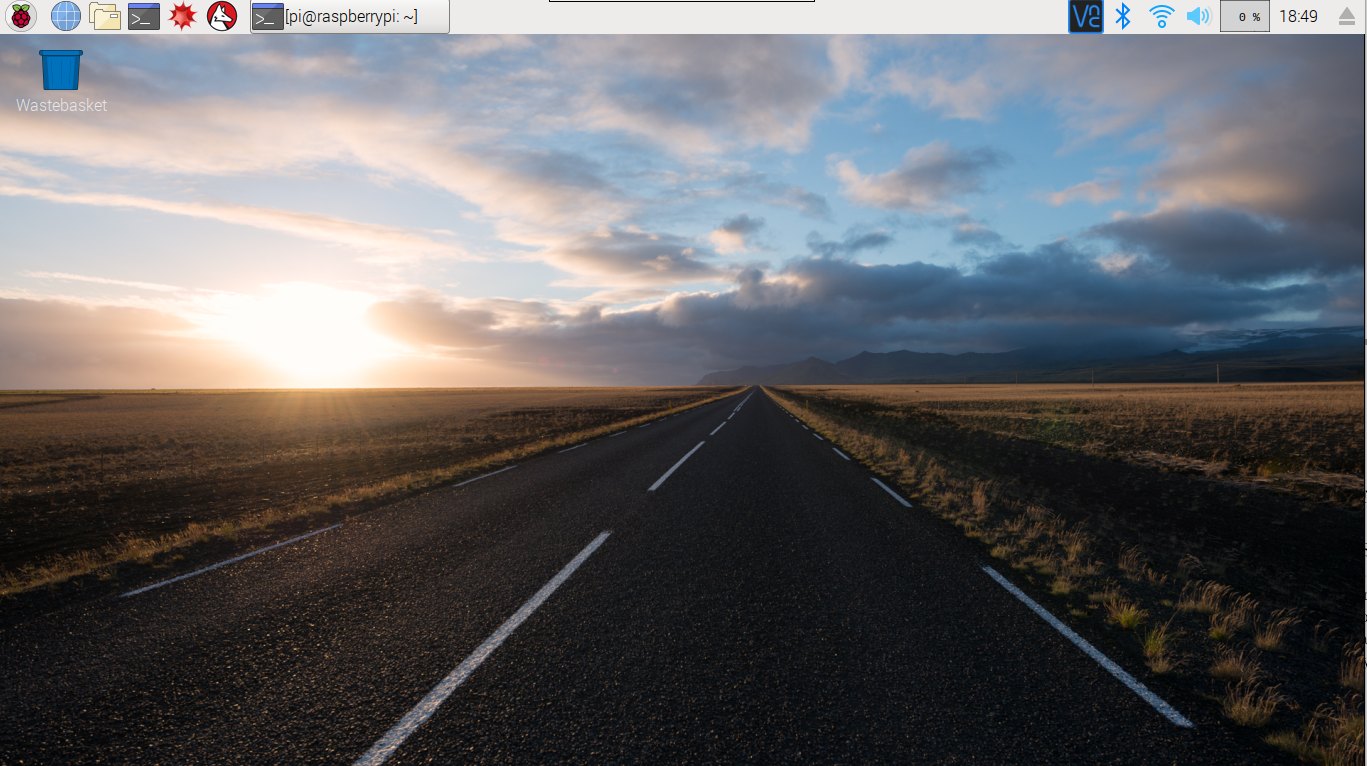
\includegraphics[width=0.8\linewidth]{img/escritorio}
	\caption{Escritorio de Raspbian Stretch en Raspberry Pi.}
	\label{fig:escritorio}
\end{figure}

Lo primero que recomiendo es actualizar el sistema y todos sus paquetes a las versiones más actuales, y activar además las opciones de VNC y SSH desde la configuración de la Raspberry Pi. Una vez hecho todo lo anterior, antes de empezar debemos comprobar que ya venga por defecto preinstalada una versión de Python 3 en nuestro sistema.\\
Para comprobarlo debemos abrir una terminal, ya sea mediante el icono de la barra de tareas o la combinación de teclas Ctrl + Alt + T.\\
Una vez dentro de la terminal, hay que tener en cuenta que el sistema contiene a la vez una versión de Python 2 y una de Python 3. Para diferenciar cuando se utiliza cada una, se sigue la siguiente norma: Siempre que un comando comience por \textit{python}, se usará la versión 2 y cuando el comando comience por \textit{python3} se usará la 3.\\
Teniendo en cuenta esta aclaración, vamos a ejecutar un comando con Python 3 para conocer la versión instalada y a su vez, comprobar que realmente exista una versión de Python 3 instalada. El comando a utilizar es el siguiente: \\ \\
\indent\verb|python3 --version| \\
La salida por pantalla de la terminal debería parecerse a la que se muestra en la imagen \ref{fig:version}.

\begin{figure}[h!]
	\centering
	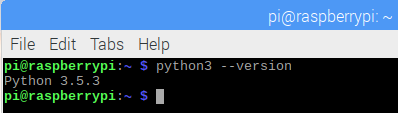
\includegraphics[width=0.8\linewidth]{img/version_python}
	\caption{Salida por pantalla del comando python3 --version.}
	\label{fig:version}
\end{figure}

Sabiendo que nuestro sistema ya tiene una versión preinstalada de Python 3, no tenemos nada más que pasar los archivos \textit{Servidor.py}, \textit{Database.py} y la carpeta \textit{imagenes} a la Raspberrry y ejecutarlos. Podemos pasarlos a través de Internet o simplemente introduciendo una memoria USB en la Raspberry con ellos.
Para que todo quede más ordenado he creado una carpeta llamada \textit{Servidor Raspberry} que contendrá todos los ficheros necesarios. Debería verse como en la imagen \ref{fig:directorio}.

\begin{figure}[h!]
	\centering
	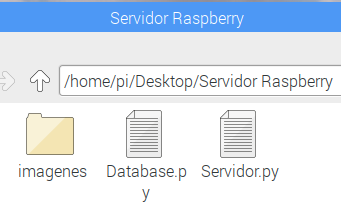
\includegraphics[width=0.8\linewidth]{img/directorio_servidor}
	\caption{Directorio \textit{Servidor Raspberry} que contiene los ficheros especificados.}
	\label{fig:directorio}
\end{figure}

\subsection{Android}\label{sec:instalacionAndroid}

Para comenzar a utilizar la aplicación, lo primero que tenemos que hacer es instalar la apk. Para poder poder instalarla, al ser una aplicación externa que no proviene de ninguna market o tienda, es necesario activar la opción de orígenes desconocidos que permite instalar aplicaciones de terceros. Para activar dicha opción tenemos que seguir los siguientes pasos:

\begin{enumerate}
	\item Entrar en el menú \textit{Ajustes} de nuestro terminal Android.
	\item Dirígete a la opción \textit{Seguridad} dentro de la categoría \textit{Personal}.
	\item Y ahora de nuevo dirígete a la sección \textit{Administración de dispositivos} y la segunda opción \textit{Orígenes desconocidos} es la que debemos activar.
	\item Una vez intentemos activarla, nos mostrará un mensaje de confirmación que deberemos aceptar. 
\end{enumerate}

La apk se puede descargar directamente desde el repositorio del proyecto (\url{https://github.com/MJ0T4/Simulador_Domotica_Raspberry}).

\section{Manual del usuario}

Es esta sección vamos a explicar detalladamente como conseguir ejecutar la parte de \textit{Raspberry Pi} y la parte de \textit{Android} conjuntamente.

\subsection{Raspberry Pi}\label{sec:ejecuciónRaspberry}

Para comenzar con la parte del servidor, he optado por introducir la IP sobre la que se creará el servidor de forma gráfica para que sea más fácil para el usuario. Lo primero es saber como ejecutar el servidor y para ello vamos a seguir los siguientes pasos:

\begin{enumerate}
	\item Abrimos una terminal desde el icono de la barra de tareas o con la combinación de teclas Ctrl + Alt + T.
	\item Necesitamos dirigirnos al \textit{Escritorio} que es donde habíamos guardado previamente los ficheros. Para ello escribimos: \\ \\
	\verb|cd Desktop/|
	\item Ahora que ya nos encontramos en el \textit{Escritorio} debemos ir a la carpeta que donde tengamos los ficheros, en mi caso \textit{Servidor Raspberry}.\\ \\
	\verb|cd Servidor\ Raspberry/|
	\item Por seguridad comprobaremos que realmente los ficheros están ahí mediante el comando \verb|ls|.
	\item Una vez hemos comprobado que tenemos los ficheros \textit{Servidor.py}, \textit{Database.py} y el directorio \textit{imagenes}, ya podemos ejecutar el servidor. Para ello utilizamos el siguiente comando:\\\\
	\verb|python3 Servidor.py|
\end{enumerate}

En la imagen \ref{fig:terminal} se puede observar una terminal con los comandos que hemos mencionado antes.

\begin{figure}[h!]
	\centering
	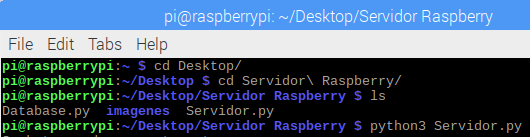
\includegraphics[width=0.9\linewidth]{img/terminal}
	\caption{Terminal con los comandos necesarios para ejecutar el servidor.}
	\label{fig:terminal}
\end{figure}

Después del último comando se abrirá una nueva ventana que será la interfaz que nos mostrará los elementos de nuestra casa que iremos creando y modificando mediante la aplicación de Android. \\
Por defecto, si la aplicación acaba de ser arrancada por primera vez, nos mostrará un error diciéndonos que no ha sido posible montar el servidor sobre esa ip. El error será igual al de la imagen \ref{fig:error}.

\begin{figure}[h!]
	\centering
	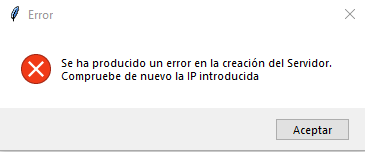
\includegraphics[width=0.8\linewidth]{img/error}
	\caption{Error en la creación del servidor esa una IP.}
	\label{fig:error}
\end{figure}

Cuando pulsemos el botón \textit{Aceptar}, se abrirá una ventana emergente en la que podremos escribir nuestra IP y que será almacenada en la base datos. Por tanto, una vez que hemos introducido nuestra IP correctamente, el resto de veces que carguemos el servidor de nuevo utilizará esta IP. \\
La ventana emergente se verá como la imagen \ref{fig:ventanaEmergente}.

\begin{figure}[h!]
	\centering
	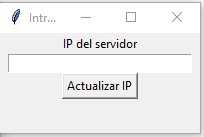
\includegraphics[width=0.4\linewidth]{img/ventanaEmergente}
	\caption{Error en la creación del servidor esa una IP.}
	\label{fig:ventanaEmergente}
\end{figure}

Una vez introducida la IP y pulsado el botón \textit{Actualizar IP}, la ventana se cerrará y se intentará crear de nuevo el servidor. Si la IP introducida es incorrecta, volverá a mostrarse el error y de nuevo la ventana emergente. Si la IP es correcta, el servidor se creará y no saltarán más errores. Si por alguna razón debiésemos reiniciar el servidor, no será necesario introducir de nuevo la IP porque ha sido guardada en la base de datos.\\
Si quisiéramos introducir una nueva IP válida, solo tendríamos que borrar la base de datos manualmente o con la opción existente en la App móvil. \\

\subsection{Android}\label{sec:manualAndroid}

Con la aplicación ya instalada, vamos a hablar sobre las posibilidades que nos ofrece la App y sus ventanas.

\subsubsection{Ventana Principal}

\begin{figure}[h!]
	\centering
	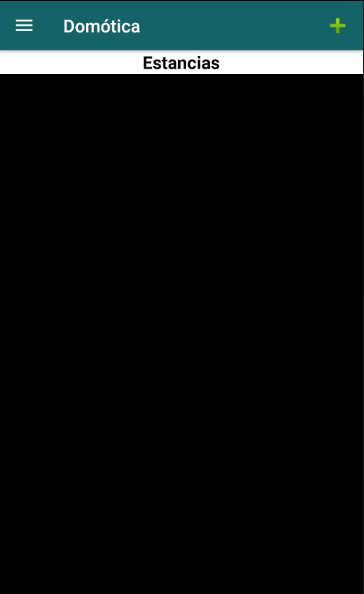
\includegraphics[width=0.35\linewidth]{img/ventanaPrincipal}
	\caption{Ventana inicial y principal de esta aplicación.}
	\label{fig:ventanaPrincipal}
\end{figure}

Cuando se abre la aplicación nos encontramos con la ventana que se muestra en la imagen \ref{fig:ventanaPrincipal}. En ella se mostrarán nuestras estancias, es decir, las diferentes salas de estar que podemos crear. Las salas que podemos crear son \textit{\textbf{Habitaciones}}, \textit{\textbf{Salones}}, \textit{\textbf{Cocinas}} y \textit{\textbf{Baños}}, y cada una de ellas tiene una imagen asignada. \\
En la parte superior, contamos con un menú desplegable que podemos mostrar pulsando sobre las tres líneas blancas horizontales, el título y un botón desde el que podemos desplegar opciones.\\
Pinchando sobre el botón con icono verde y símbolo \textbf{+} se mostrará una ventana emergente con diferentes opciones. En dicha ventana \ref{fig:opcionesEstancias}, tendremos la opción de crear cualquier tipo de las cuatro estancias pulsando sobre su nombre y además elegir un nombre para ella. \\

\begin{figure}[h!]
	\centering
	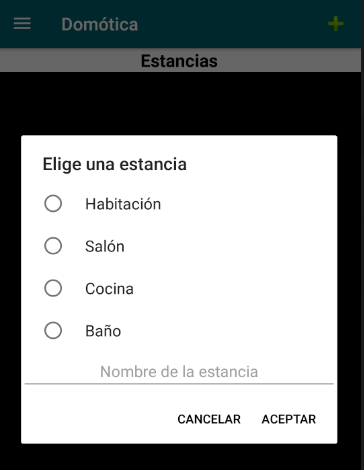
\includegraphics[width=0.4\linewidth]{img/opcionesEstancias}
	\caption{Ventana emergente para la creación de nuevas estancias.}
	\label{fig:opcionesEstancias}
\end{figure}

Tras seleccionar una de las opciones y escribir un nombre para ella, pulsamos sobre el botón \textit{Aceptar} y se creará. Para realizar un ejemplo, crearemos una \textit{Habitación} con el nombre \textit{Habitación}, que podremos ver en la imagen \ref{fig:creacionHabitacion}. \\

\begin{figure}[h!]
	\centering
	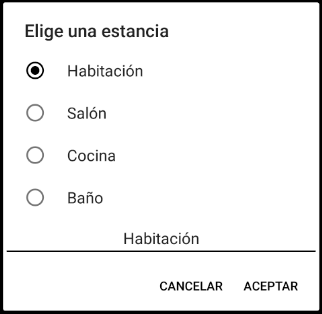
\includegraphics[width=0.5\linewidth]{img/creacionHabitacion}
	\caption{Creación de una nueva \textit{Habitación} mediante la ventana emergente.}
	\label{fig:creacionHabitacion}
\end{figure}

Una vez pulsado el botón \textit{Aceptar} se nos creará la habitación y la ventana principal se nos quedará de la siguiente manera \ref{fig:ventanaPrincipalHabitacion}.\\
Con está habitación ya creada, contamos con las opciones de eliminarla o cambiar su nombre.

\begin{figure}[h!]
	\centering
	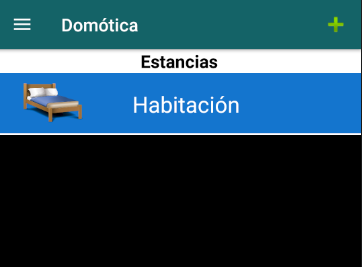
\includegraphics[width=0.5\linewidth]{img/ventanaPrincipalHabitacion}
	\caption{Creación de una nueva \textit{Habitación} mediante la ventana emergente.}
	\label{fig:ventanaPrincipalHabitacion}
\end{figure}

Para poder borrar o cambiar el nombre de la \textit{Habitación} creada anteriormente debemos acceder a su menú contextual. Este menú aparecerá tras pulsar poco más de un segundo sobre ella. Se puede ver en la imagen \ref{fig:menuContextual}.

\begin{figure}[h!]
	\centering
	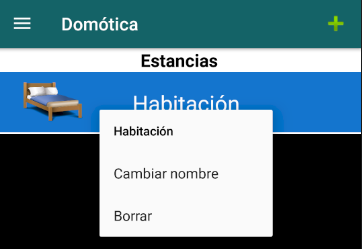
\includegraphics[width=0.6\linewidth]{img/menuContextual}
	\caption{Menú contextual de una estancia}
	\label{fig:menuContextual}
\end{figure}

Si pulsamos sobre la opción \textit{Cambiar nombre} se mostrará una nueva ventana emergente en la que debemos insertar el nombre y pulsar el botón \textit{Aceptar}. Dicha ventana emergente se verá como la imagen \ref{fig:cambiarNombre}

\begin{figure}[h!]
	\centering
	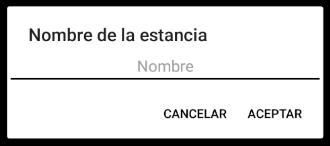
\includegraphics[width=0.6\linewidth]{img/cambiarNombre}
	\caption{Opción \textit{Cambiar nombre} del menú contextual de una \textit{Habitación}.}
	\label{fig:cambiarNombre}
\end{figure}

En cambio, si pulsamos sobre la opción \textit{Borrar} se mostrará un mensaje emergente de confirmación para la realización de dicha acción. El mensaje sería igual al de la imagen \ref{fig:borrar}.

\begin{figure}[h!]
	\centering
	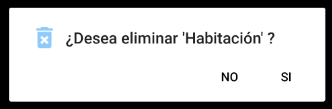
\includegraphics[width=0.6\linewidth]{img/borrar}
	\caption{Opción \textit{Borrar} del menú contextual de una \textit{Habitación}.}
	\label{fig:borrar}
\end{figure}

Para poder realizar todas las acciones a anteriores es necesario estar conectado al servidor, sino se nos mostrará una ventana emergente \ref{fig:ventanaEmergenteError} con un botón que nos dirigirá a la ventana del Servidor. 

\begin{figure}[h!]
	\centering
	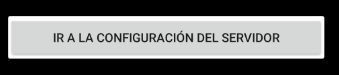
\includegraphics[width=0.6\linewidth]{img/ventanaEmergenteError}
	\caption{Ventana emergente en caso de no estar conectado al servidor.}
	\label{fig:ventanaEmergenteError}
\end{figure}

Si pulsamos sobre las tres líneas blancas horizontales en la barra superior, se desplegará un menú. En este menú tenemos dos opciones:

\begin{itemize}
	\item \textbf{Servidor}, que nos redirigirá a la misma ventana que el botón de la imagen \ref{fig:ventanaEmergenteError}.
	\item \textbf{Borrar base de datos}, que borrará tanto los datos locales como los del servidor.
\end{itemize}

El menú desplegable podemos verlo en la imagen \ref{fig:menuPrincipal}.

\begin{figure}[h!]
	\centering
	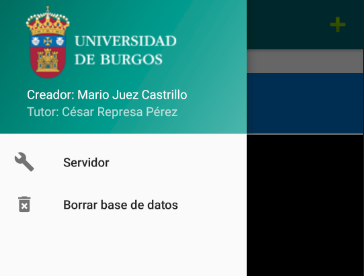
\includegraphics[width=0.6\linewidth]{img/menuPrincipal}
	\caption{Menú principal que se mostrará al pulsar en las tres líneas blancas horizontales}
	\label{fig:menuPrincipal}
\end{figure}

\subsubsection{Ventana Servidor}

Esta es otra de las ventanas de la aplicación desde la que podemos acceder mediante el menú desplegable que se encuentra en la ventana principal(\ref{fig:menuPrincipal}) o mediante el botón de la ventana emergente que se nos muestra cuando queremos realizar una acción y no estamos conectados al servidor (\ref{fig:ventanaEmergenteError}).\\

En la ventana servidor (\ref{fig:servidor}) nos encontramos con dos campos para rellenar:

\begin{figure}[h!]
	\centering
	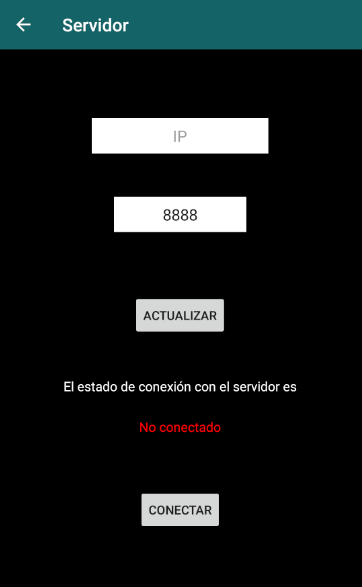
\includegraphics[width=0.6\linewidth]{img/servidor}
	\caption{Ventana \textit{Servidor} de la aplicación.}
	\label{fig:servidor}
\end{figure}

\begin{itemize}
	\item \textbf{IP}, este campo viene vacío por defecto y en él debemos escribir la \textit{IP} del servidor al que queremos conectarnos.
	\item \textbf{Puerto}, este campo viene por defecto como \textbf{8888} y es el puerto que se usará para realizar la conexión, aunque permite la posibilidad de ser cambiado.
\end{itemize}

Una vez hemos escrito la \textbf{IP} y el \textbf{Puerto} al que deseamos conectarnos, solo debemos presionar el botón \textit{Actualizar}. Cuando el botón es pulsado, estos datos son guardados en la base de datos para futuras conexiones, de manera que solo deberíamos realizar este paso una vez. \\
Tras actualizar los datos, ya podemos conectarnos al servidor, así que pulsamos sobre el botón \textit{Conectar} que se encuentra en la inferior. Si la conexión se ha realizado con éxito, nuestra ventana del Servidor se debería ver como la imagen \ref{fig:conectado}, sino se seguiría viendo como la imagen \ref{fig:servidor}.

\begin{figure}[h!]
	\centering
	\includegraphics[width=0.6\linewidth]{img/conectado}
	\caption{Conexión exitosa con el servidor.}
	\label{fig:conectado}
\end{figure}

Esta acción de conectarse al servidor solo deberá realizarse una vez, ya que por defecto en la ventana principal \ref{fig:ventanaPrincipal} tratará de conectarse al servidor con la \textbf{IP} que hayamos guardado en la base de datos desde la ventana del Servidor \ref{fig:servidor}.

Una vez estamos conectados y deseamos volver a la ventana principal, solo debemos pulsar sobre la flecha que se encuentra en la parte superior izquierda de la ventana. De nuevo en ventana principal, vamos a hablar sobre la última ventana.

\subsubsection{Ventana iluminación}

La ventana de iluminación es una ventana desde la cuál podemos crear, modificar y eliminar \textit{Bombillas} para las estancias creadas en la ventana principal. Para acceder a ella, solo debemos encontrarnos en la ventana principal y pulsar sobre la estancia que queremos. Tras esto, nos dirigirá a una nueva ventana como la de la imagen \ref{fig:ventanaIluminacion}

\begin{figure}[h!]
	\centering
	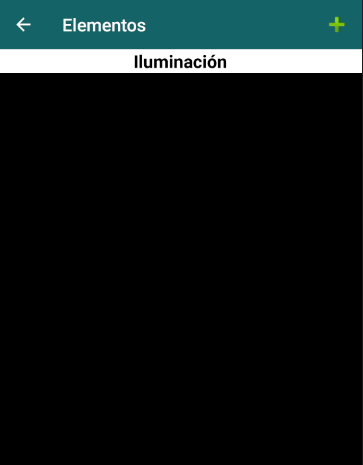
\includegraphics[width=0.6\linewidth]{img/ventanaIluminacion}
	\caption{Ventana iluminación.}
	\label{fig:ventanaIluminacion}
\end{figure}

Pinchando sobre el botón con icono verde y símbolo \textbf{+} que se encuentra en la parte superior derecha, se mostrará una ventana emergente \ref{fig:ventanaEmergenteBombilla} para la creación de bombillas. 

\begin{figure}[h!]
	\centering
	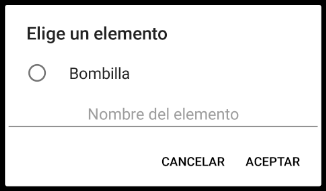
\includegraphics[width=0.6\linewidth]{img/ventanaEmergenteBombilla}
	\caption{Ventana emergente para la creación de una bombilla.}
	\label{fig:ventanaEmergenteBombilla}
\end{figure}

Debemos pinchar sobre la única opción posible, especificar un nombre para ella y pulsar sobre el botón \textit{Aceptar}. Tras hacerlo, se nos creará una nueva \textit{Bombilla} y nuestra ventana de iluminación se verá como la de la imagen \ref{fig:ventanaIluminacion2}.

\begin{figure}[h!]
	\centering
	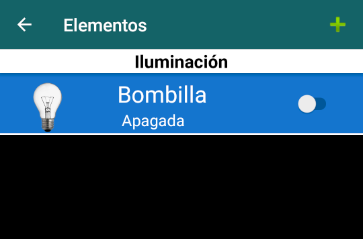
\includegraphics[width=0.6\linewidth]{img/ventanaIluminacion2}
	\caption{Ventana iluminación tras crear una \textit{Bombilla}.}
	\label{fig:ventanaIluminacion2}
\end{figure}

En esta nueva \textit{Bombilla} contamos con una imagen, que nos muestra su estado, su nombre, un texto que también que nos indica su estado y un interruptor para encenderla y apagarla. Para cambiar su estado, es tan sencillo como pulsar el interruptor y ver como se ilumina la bombilla, tanto aquí como en la parte de Python. La imagen \ref{fig:bombillaIluminada} muestra como sería el resultado de pulsar el interruptor.

\begin{figure}[h!]
	\centering
	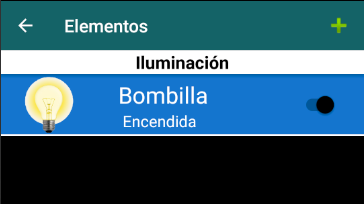
\includegraphics[width=0.6\linewidth]{img/bombillaIluminada}
	\caption{Ventana iluminación con una \textit{Bombilla} encendida.}
	\label{fig:bombillaIluminada}
\end{figure}

Además de todo esto, cada \textit{Bombilla} que creemos, contará con su propio menú contextual \ref{fig:menuContextualBombilla} con las mismas opciones que las estancias (\textit{Cambiar nombre} y \textit{Borrar})  y que se mostrará de la misma manera.

\begin{figure}[h!]
	\centering
	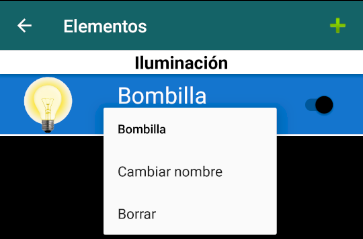
\includegraphics[width=0.6\linewidth]{img/menuContextualBombilla}
	\caption{Menú contextual de una \textit{Bombilla}.}
	\label{fig:menuContextualBombilla}
\end{figure}


\bibliographystyle{plain}
\bibliography{bibliografiaAnexos}

\end{document}
